\documentclass[a4paper]{article}
\usepackage[spanish]{babel}
\usepackage[utf8]{inputenc}
\usepackage{graphicx}
\usepackage{enumerate}
\usepackage{listings}
\usepackage{color}
\usepackage{indentfirst}
\usepackage{fancyhdr}
\usepackage{latexsym}
\usepackage{blkarray}
\usepackage{multirow}
\usepackage[colorlinks=true, linkcolor=black]{hyperref}
%\usepackage{makeidx}
%\usepackage{float}
\usepackage{calc}
\usepackage{amsmath, amsthm, amssymb}
\usepackage{amsfonts}
%\lstset{language=C}
\definecolor{gray}{gray}{0.5}
\definecolor{light-gray}{gray}{0.95}
\definecolor{orange}{rgb}{1,0.5,0}

\usepackage{fancyhdr}
\pagestyle{fancy}

%\renewcommand{\chaptermark}[1]{\markboth{#1}{}}
\renewcommand{\sectionmark}[1]{\markright{\thesection\ - #1}}

\fancyhf{}

\fancyhead[LO]{Sección \rightmark} % \thesection\
\fancyfoot[RO]{\thepage}
\renewcommand{\headrulewidth}{0.5pt}
\renewcommand{\footrulewidth}{0.5pt}
\setlength{\hoffset}{-0.8in}
\setlength{\textwidth}{16cm}
%\setlength{\hoffset}{-1.1cm}
%\setlength{\textwidth}{16cm}
\setlength{\headsep}{0.5cm}
\setlength{\textheight}{25cm}
\setlength{\voffset}{-0.7in}
\setlength{\headwidth}{\textwidth}
\setlength{\headheight}{13.1pt}

\renewcommand{\baselinestretch}{1.1}  % line spacing


% \setcounter{secnumdepth}{2}
\usepackage{underscore}
\usepackage{caratula}
\usepackage{url}
\usepackage{float}

\usepackage{commath}
\usepackage[draft]{todonotes}
\usepackage{caption}

\usepackage{algorithm}
\usepackage[noend]{algpseudocode}
\usepackage{array}
\usepackage{xcolor,colortbl}
\usepackage{amsthm}
\usepackage{mathtools}
\usepackage{listings}
\usepackage{svg}
\usepackage{systeme}
\usepackage{color,soul}

\captionsetup[figure]{labelformat=empty}% redefines the caption setup of the figures environment in the beamer class.
\makeatletter
\renewcommand*\env@matrix[1][*\c@MaxMatrixCols c]{%
  \hskip -\arraycolsep
  \let\@ifnextchar\new@ifnextchar
  \array{#1}}
\makeatother


\newcommand{\cod}[1]{{\tt #1}}
\newcommand{\negro}[1]{{\bf #1}}
\newcommand{\ital}[1]{{\em #1}}
\newcommand{\may}[1]{{\sc #1}}
\newcommand{\tab}{\hspace*{2em}}

\hypersetup{
 pdfstartview= {FitH \hypercalcbp{\paperheight-\topmargin-1in-\headheight}},
 pdfauthor={Grupo},
 pdfsubject={Dise\~{n}o}
}

\lstdefinestyle{customc}{
  backgroundcolor=\color{light-gray},
  belowcaptionskip=1\baselineskip,
  breaklines=true,
  numbers=left,
  xleftmargin=\parindent,
  language=C,
  showstringspaces=false,
  basicstyle=\footnotesize\ttfamily,
  keywordstyle=\bfseries\color{blue},
  commentstyle=\itshape\color{gray},
  identifierstyle=\color{black},
  stringstyle=\color{orange},
}

\lstdefinestyle{customasm}{
  backgroundcolor=\color{light-gray},
  belowcaptionskip=1\baselineskip,
  numbers=left,
  xleftmargin=\parindent,
  language=[x86masm]Assembler,
  keywordstyle=\bfseries\color{blue},
  basicstyle=\footnotesize\ttfamily,
  commentstyle=\itshape\color{gray},
}

\lstset{escapechar=@}


\begin{document}

\thispagestyle{empty}
\materia{Métodos Númericos}
\submateria{2do Cuatrimestre - 2017}
\titulo{Trabajo Práctico I}
% \subtitulo{Subtitulo}
\integrante{Jonathan Seijo}{592/15}{jon.seijo@gmail.com}
\integrante{Lucas De Bortoli}{736/15}{lu_cas_.97@hotmail.com.ar}
\integrante{COMPLETAR}{COMPLETAR}{COMPLETAR}
\integrante{COMPLETAR}{COMPLETAR}{COMPLETAR}

\makeatletter

\maketitle
\newpage

\thispagestyle{empty}
\vfill

\thispagestyle{empty}
\vspace{3cm}
\tableofcontents
\newpage

\newenvironment{myindentpar}[1]
{\begin{list}{1}
         {\setlength{\leftmargin}{#1}}
         \item[]
}
{\end{list} }

%\normalsize
\newpage

% -------------------------------------------------------
% Introducción Teórica
% -------------------------------------------------------
\section{Introducción}

% Pautas de tp hablan de "brave introduccion"

Este trabajo consiste en la digitalización de objetos 3D basándose en imágenes producidas con cámaras tradicionales, utilizando la técnica de \textit{fotometría estéreo}. Mostraremos que utilizando luces provenientes de diferentes ángulos, podemos aproximar las normales a la superficie y estimar las profundidades de cada punto.

Para esto debemos resolver varios sistemas de ecuaciones lineales, los cuáles resolveremos algorítmicamente de forma matricial. Usaremos en un primer caso el método clásico de Eliminación Gaussiana, y veremos como utilizando factorización LU podemos reducir los tiempos de cómputo. Luego, utilizaremos la factorización de Cholesky.

Los experimentos .... []
\todo[inline]{Completar breve pantallazo a experimentos}

% -------------------------------------------------------
% Calibracion
% -------------------------------------------------------
\newpage

% Template de matriz
% \[
% \begin{bmatrix} % Matriz con linea rectangular
% \begin{pmatrix} % Matriz con linea redonda
%     x_{11} & x_{12} & x_{13} & \dots  & x_{1n} \\
%     x_{21} & x_{22} & x_{23} & \dots  & x_{2n} \\
%     \vdots & \vdots & \vdots & \ddots & \vdots \\
%     x_{d1} & x_{d2} & x_{d3} & \dots  & x_{dn}
% \end{pmatrix}
% \end{bmatrix}
% \]

\section{Calibración}

El paso anterior al cálculo de las profundidades es el cálculo de los vectores normales a todo punto de la superficie. Para esto, se eligen tres luces diferentes (por ejemplo si elegimos 1, 2 y 3, nuestros vectores luz serán $s^{1}$, $s^{2}$ y $s^{3}$ respectivamente) y utilizando las intensidades ya registradas ($I_i$) queremos encontrar los $m$ que son solución, donde $m$ es un vector que depende del vector normal y de una constante del objeto. Cabe aclarar que el sistema se deberá resolver para cada píxel de la imagen, por lo que ya conocemos las intensidades del píxel dado para toda imagen. Nos encontramos entonces con el primer problema, porque los vectores de luz no son un dato conocido. \\

El sistema que queremos resolver es el siguiente: \\

\[
% \begin{bmatrix} % Matriz con linea rectangular
\begin{pmatrix}
    s_{x}^{1} & s_{y}^{1} & s_{z}^{1} \\
    s_{x}^{2} & s_{y}^{2} & s_{z}^{2} \\
    s_{x}^{3} & s_{y}^{3} & s_{z}^{3}
\end{pmatrix}
% \end{bmatrix}
\begin{pmatrix}
    m_{x} \\
    m_{y} \\
    m_{z}
\end{pmatrix}
=
\begin{pmatrix}
    I_{1} \\
    I_{2} \\
    I_{3}
\end{pmatrix}
\]

Pero no conocemos los $s_{j}^{i}$. \\

Tenemos que $S = (s_{x}^{i}, s_{y}^{i}, s_{z}^{i})$ es el vector luz en la imagen $i$. Dado que vamos a explicar el cálculo para una imagen cualquiera, omitiremos el supraíndice $i$ para una notación más relajada.

Llamemos $c = (c_{x}, c_{y}, c_{z})$ al centro de la esfera. Pensemos la luz como un vector que apunta hacia el centro. El vector $S$ toca la superficie en un cierto punto $p = (p_{x}, p_{y}, p_{z})$, pero $p$ no es un punto al azar, sino que es el punto más iluminado de la esfera. Por lo tanto, la dirección de luz que nos interesa es $S =  c - p$.\\

{\centering
    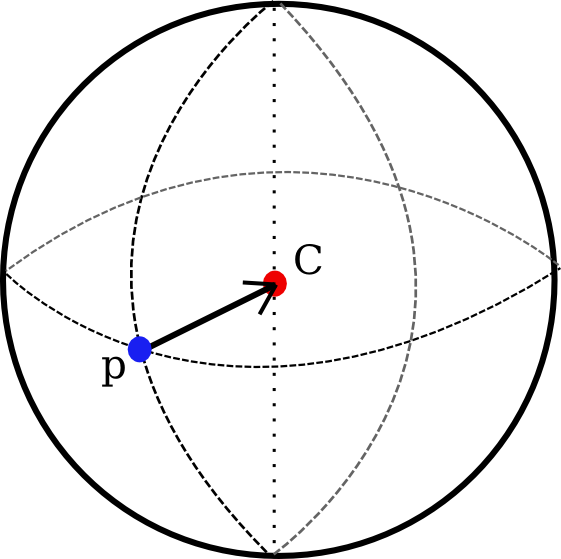
\includegraphics[scale=0.9]{informe/imagenes/esfera/esferaModelo.png} \\
    \captionof{figure}{Imagen del vector que nos interesa, $S = c - p$}
}

$ $\newline

Más precisamente, $S = (c_{x} - p_{x}, c_{y} - p_{y}, c_{z} - p_{z}).$ En principio no conocemos ninguno de estos valores, pero concentrémonos en calcular sobre el eje $x$ e $y$. De la imagen de la esfera (2D) podemos conocer algunos datos. En la implementación utilizamos la máscara provista por la cátedra para simplificar los cálculos. \\

Como los píxeles en la máscara son blancos o negros, es muy sencillo identificar los puntos que pertenecen a la esfera con sólo ver su color. Recorriendo todos los puntos y tomando máximos y mínimos obtenemos 4 puntos clave: El punto del círculo que está más arriba $A$, el más abajo $A'$, el de más a la izquierda $B$ y el de más a la derecha $B'$. \\

{\centering
    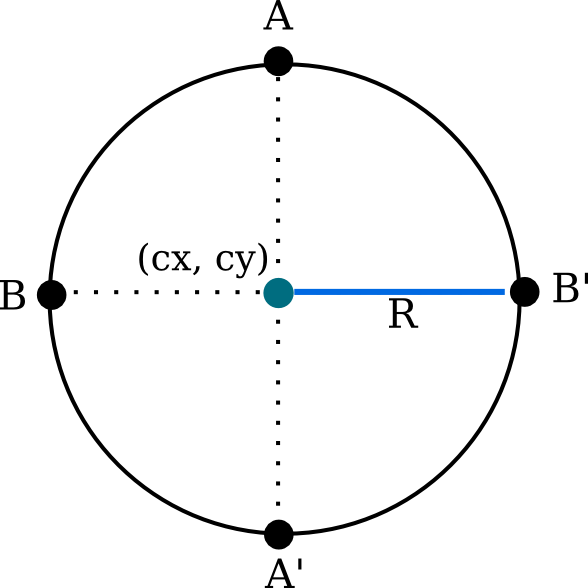
\includegraphics[scale=0.5]{informe/imagenes/esfera/circulo.png} \\
}

Puede verse fácilmente que el radio $R$ del círculo es la mitad de la distancia entre $B$ y $B'$

\begin{center}
$R = \frac{|B'_x - B_x|}{2}$.
\end{center}

Además, sabiendo que $c$ es el centro del círculo,

\begin{center}
    $c_{x} = B_x + R$ \\
    $c_{y} = A_y + R$
\end{center}

Necesitamos encontrar también quién es $p$. Una primera idea fue recorrer todos los píxeles y quedarnos con el de mayor intensidad. Esto nos trajo problemas pues en una imagen no hay un único píxel más brillante que el resto, sino que existe un pequeño sector que se encuentra más iluminado. Nos encontramos con imágenes diferentes (pero con similares intensidades de luz) para los cuales se calculaba el mismo punto $p$. \\

Para resolver esto consideramos para cada píxel una pequeña vecindad (en principio de 5 x 5, pero se fueron probando otras) y nos quedamos con el píxel que tuviese la vecindad más iluminada. Utilizando este método podemos hallar el $p = (p_x, p_y)$ que queríamos. \\

Tenemos entonces los datos de $c_x$, $c_y$, $p_x$, $p_y$ y $R$. Veamos cómo podemos despejar lo que nos falta. Recordemos lo que queríamos calcular:
\begin{center}
    $S = (c_{x} - p_{x}, c_{y} - p_{y}, c_{z} - p_{z}).$
\end{center}

Sólo la tercer componente de $S$ es una incógnita. Sabemos que el radio del círculo es igual al radio de la esfera y el radio de la esfera es igual a la distancia euclidea entre el centro y un punto en la superficie. En particular, el radio es igual a la distancia entre $p$ y $c$. Es decir:

\begin{center}
    $\norm{c - p} = R$ \\
\end{center}

Despejando,

\begin{center}
    $\sqrt{(c_{x} - p_{x})^{2} + (c_{y} - p_{y})^{2} + (c_{z} - p_{z})^{2}} = R$ \\ $ $

    $(c_{x} - p_{x})^{2} + (c_{y} - p_{y})^{2} + (c_{z} - p_{z})^{2} = R^{2}$ \\ $ $

    $(c_{z} - p_{z})^{2} = R^{2} - (c_{x} - p_{x})^{2} - (c_{y} - p_{y})^{2}$ \\ $ $

    $(c_{z} - p_{z}) = \sqrt{R^{2} - (c_{x} - p_{x})^{2} - (c_{y} - p_{y})^{2}}$ \\ $ $

\end{center}

Finalmente conseguimos lo que buscábamos. Repitiendo este procedimiento, podemos obtener todas las componentes del vector de luz para todas las imagenes. Podemos escribir a cualquier vector de luz utilizando datos conocidos:

\begin{center}
    $s_x = c_{x} - p_{x}$ \\
    $s_y = c_{y} - p_{y}$ \\
    $s_z = \sqrt{R^{2} - (c_{x} - p_{x})^{2} - (c_{y} - p_{y})^{2}})$ \\
\end{center}

Ya estamos en condiciones de resolver el sistema original pues conocemos todos sus coeficientes. Analizaremos en las siguientes secciones diferentes formas para resolverlo.




% -------------------------------------------------------
% Desarrollo
% -------------------------------------------------------
\newpage
% Cita textual seccion Desarrolo:

% Deben explicarse los metodos numericos que utilizaron
% y su aplicacion al problema concreto involucrado en el trabajo practico.
% Se deben mencionar los pasos que siguieron para implementar
% los algoritmos, las dificultades que fueron encontrando y la
% descripcion de como las fueron resolviendo.

% Explicar tambien como fueron planteadas y realizadas las
% mediciones experimentales. Los ensayos fallidos, hipotesis y
% conjeturas equivocadas, experimentos y metodos malogrados deben
% figurar en esta seccion,
% con una breve explicacion de los motivos de estas fallas
% (en caso de ser conocidas).

\section{Cálculo de normales}

En esta sección resolveremos el problema de calcular los vectores normales a la superficie, conociendo los vectores luz y los valores de la intensidad para cada píxel dado. Resolveremos utilizando el algoritmo de eliminación gaussiana, y veremos en la siguiente sección una forma de optimizar los cálculos aprovechándonos de las propiedades de nuestro problema.

\subsection{Eliminación Gaussiana}

Para cada píxel, tenemos un sistema listo para resolver:

% Sistema de matrices original
\[
\begin{pmatrix}
    s_{x}^{1} & s_{y}^{1} & s_{z}^{1} \\
    s_{x}^{2} & s_{y}^{2} & s_{z}^{2} \\
    s_{x}^{3} & s_{y}^{3} & s_{z}^{3}
\end{pmatrix}
\begin{pmatrix}
    m_{x} \\
    m_{y} \\
    m_{z}
\end{pmatrix}
=
\begin{pmatrix}
    I_{1} \\
    I_{2} \\
    I_{3}
\end{pmatrix}
\]

Donde cada $s_{c}^{i}$ es la coordenada $c$ del vector de luz en la imagen $i$, los $I_i$ las intensidades de luz (del píxel actual) en la imagen $i$, y los $m_j$ nuestras incógnitas. El vector $m = (m_x, m_y, m_z)$ no es exactamente el valor de la normal $n$, sino que $m = I_0 \rho . n$, con $I_0, \rho \in \mathbb{R}$ constantes desconocidas que dependen del objeto. Lo que nos interesa es encontrar el valor de $n$, pero para esto primero debemos hallar $m$. \\

La pregunta ahora es ¿cómo lo resolvemos?. Dado que en principio no sabemos cómo, nos gustaría llevarlo a una forma equivalente que sea mas fácil de resolver. Podemos hacer esta conversión a un sistema equivalente usando el algoritmo de eliminación de Gauss. Lo que hace este algoritmo es llevar una matriz a su forma triangular superior, de dónde luego es muy sencillo hacer los despejes finales. \\

El pseudocódigo del algoritmo de Gauss es el siguiente:

\begin{algorithm}[H]
\begin{algorithmic}
\Function{EliminacionGaussiana}{Matriz M[$n$][$m$]}

    \For{$k \in [1..min(n,m)]$ }
        \For{$i \in [k+1..m]$ }

            \If{$\|$M[$k$][$k$]$\|$ $> \epsilon$}
                \State $mult \gets $M[$i$][$k$] $/$ M[$k$][$k$]
                \For{$j \in [k+1..n]$}

                    \State M[$i$][$j$] $\gets$ M[$i$][$j$] - mult*M[$k$][$j$]

                \EndFor
            \Else
                \State Hay un cero en la diagonal!
            \EndIf
        \EndFor
    \EndFor

\EndFunction
\end{algorithmic}
\end{algorithm}

Como puede verse, funciona correctamente sólo \textbf{suponiendo que no hay ceros en la diagonal}. Es claro que puede modificarse para que realice intercambios de filas y no tenga el problema del cero, pero veremos que para nuestro problema no es importante. En nuestra implementación aplicaremos el algoritmo de Gauss en la siguiente matriz ampliada:

% Matriz ampliada
\[
\begin{pmatrix}[ccc|c]
    s_{x}^{1} & s_{y}^{1} & s_{z}^{1} & I_{1} \\
    s_{x}^{2} & s_{y}^{2} & s_{z}^{2} & I_{2} \\
    s_{x}^{3} & s_{y}^{3} & s_{z}^{3} & I_{3}
\end{pmatrix}
\]

Para empezar, nuestros $s_{j}^{i}$ incialmente son todos distintos de cero, asi que nunca habrá un cero en la primer fila. Dado que son sólo 12 vectores de luces, tomamos todas las posibles combinaciones de tres luces y corrimos el algoritmo de gauss sin pivoteos. En ningun caso se realizó división por cero ni tampoco apareció ningún cero en la diagonal. El código de lo realizado puede encontrarse en \textit{TestTieneLU.cpp}. Esto cobrará importancia cuando querramos encontrar factorización LU. \\

Dado que pudimos triangular correctamente la matriz ampliada, entonces ya estamos en condiciones de despejar nuestra matriz extendida de 3 x 4:

\[
\begin{pmatrix}[ccc|c]
    a_{1,1}   & a_{1,2} & a_{1,3} & a_{1, 4} \\
    0         & a_{2,2} & a_{2,3} & a_{2, 4} \\
    0         & 0       & a_{3,3} & a_{3, 4}
\end{pmatrix}
\]

\begin{algorithm}[H]
\begin{algorithmic}

\Function{Despejar}{Matriz M[$n$][$m$]}

    // En X se guardan los m-1 coeficientes solución (Recordemos que M es ampliada)
    \State X[$m-1$] $\gets \{\}$ \\

    \For{$j \in [1..m-1]$ }  (j es indice de columna)

        \If{$\|$M[$j$][$j$]$\|$ $> \epsilon$}

            \State X[$j$] $\gets$ M[$j$][$m$] / M[$j$][$j$]

            \For{$i \in [j-1 .. 0]$ }  (i es indice de fila)

                \State M[$i$][$m$] $\gets$ M[$i$][$m$] - ( M[$i$][$j$] * X[$j$] )

            \EndFor

        \Else
            \State Hay un cero en la diagonal!
        \EndIf
    \EndFor

    \State Retornar X

\EndFunction
\end{algorithmic}
\end{algorithm}

Resolviendo el sistema con la forma expuesta, obtenemos el vector solución $m$. Pero $m$ no es lo que buscábamos, sino que queremos obtener el valor de $n$. Recordemos:

\begin{center}
$m = I_0 \rho . (n_x, n_y, n_z) = I_0 \rho . n$
\end{center}

Con $I_0 \rho \in \mathbb{R}$. Tomando norma:

\begin{center}
$\norm{m} = \abs{I_0 \rho} \norm{n}$
\end{center}

Pero $\norm{n} = 1$, pues queremos el vector unitario. Entonces:

\begin{center}
$\norm{m} = \abs{I_0 \rho}$
\end{center}

Sabiendo esto, podemos despejar y obtener el valor de $n$ (con $m \neq 0$):

\begin{center}
$n = \frac{m}{\norm{m}}$
\end{center}

Obtuvimos así para cada píxel el vector normal a la superficie.

\subsection{Factorización LU}

Recordemos nuestro sistema para hallar las normales:
\[
\begin{pmatrix}
    s_{x}^{1} & s_{y}^{1} & s_{z}^{1} \\
    s_{x}^{2} & s_{y}^{2} & s_{z}^{2} \\
    s_{x}^{3} & s_{y}^{3} & s_{z}^{3}
\end{pmatrix}
\begin{pmatrix}
    m_{x} \\
    m_{y} \\
    m_{z}
\end{pmatrix}
=
\begin{pmatrix}
    I_{1} \\
    I_{2} \\
    I_{3}
\end{pmatrix}
\]

Una vez fijas las luces a utilizar (en este caso 1,2 y 3) para despejar la normal en cada píxel, debemos resolver el sistema en cada píxel. Es decir, estaremos traingulando una y otra vez una matriz dónde lo único que cambia es el término a la derecha de la igualdad. Por lo tanto, es interesante plantearse si existe una forma de evitar aplicar Gauss en cada punto. \\

La factorización LU podría no existir, pero veamos de qué se trata. Dada una matriz $A$, la factorización LU consiste en encontrar dos matrices: una matriz $L$ triangular inferior con unos en la diagonal y una matriz $U$ triangular superior, de forma que se cumpla

\begin{center}
$A$ = $L$.$U$
\end{center}

% Quiza explicar mejor esto
Por lo visto en clase, puede demostrarse que la $L$ tiene en la diagonal unos, ceros por arriba, y por debajo los multiplicadores que se utilizaron en la eliminación Gaussiana para colocar un cero en la triangulación. En la $U$ se colocan ceros debajo de la diagonal y en el resto los coeficientes que quedaron en la matriz ya triangulada. \\

Digamos entonces que ya conocemos la factorización LU para una matriz dada, ¿Cómo la utilizamos para resolver nuestro sistema?

\begin{center}
    $Ax = b$ $\iff$ $LUx = b$
\end{center}

Si consideramos $Ux = y$, nos queda para resolver:

\begin{center}
    $Ly = b$
\end{center}

Donde $L$ es triangular inferior. Por lo tanto podemos despejar y obtener $y$ sin necesidad de aplicar eliminación Gaussiana. Una vez que conocemos $y$, como $U$ también esta triangulada despejamos en:

\begin{center}
    $Ux = y$
\end{center}

Obteniendo así el $x$ que queríamos encontrar inicialmente. \\

Por lo expuesto en la sección anterior, experimentalmente comprobamos que en nuestra matriz de luces podemos aplicar Gauss normalmente sin encontrarnos con ceros en la diagonal y sin tener que hacer ninguna permutación de filas. \\

Por lo visto en la clase teórica, si podemos triangular una matriz usando Gauss sin tener que permutar filas, es suficiente para afirmar que la factorización LU existe, entonces con el procedimiento explicado podemos hallar la descomposicion de nuestra matriz de luces y resolver el sistema más eficientemente. \\

\newpage
\section{Estimación de profundidades}

Utilizando los métodos anteriores pudimos resolver el sistema que incluye las luces y calcular las normales para todo píxel de la imagen. Recordemos que para un cierto píxel $(a, b)$ la normal en ese punto es de la forma:

\begin{center}
$n^{(a,b)} = (n_{x}^{a,b}, n_{y}^{a,b}, n_{z}^{a,b})$
\end{center}

A partir de aquí en ocasiones omitiremos el supraíndice $(a,b)$ para relajar la notación cuando es claro cuál es el píxel del cual hablamos. Siguiendo con la técnica de fotometría estéreo, el siguiente paso a realizar es el cálculo de las profundidades utilizando estas normales. Para esto, consideramos una aproximación al plano tangente de cada píxel. Las ecuaciones que tenemos que resolver son las siguientes, para cada píxel $(x ,y)$:

\begin{center}
\[
    \begin{dcases}
        n_{y} +  n_{z} * (z_{x, y+1} - z_{x, y}) = 0 \\
        n_{x} +  n_{z} * (z_{x+1, y} - z_{x, y}) = 0
    \end{dcases}
\]
\end{center}
O equivalentemente
\begin{center}
\[\begin{dcases}
        n_{z} * z_{x, y+1} - n_{z} *  z_{x, y} = n_{y}  \\
        n_{z} * z_{x+1, y} - n_{z} *  z_{x, y} = n_{x}
    \end{dcases}
\]
\end{center}

Consideremos cómo sería el sistema matricial para una imagen de 2x3 pixeles, y veremos cómo puede generalizarse: \\

% \dots \ddots \vdots

\[
\underbrace{
\begin{pmatrix}
    % - n_{z}^{1,1}  &  0                      & 0  & n_{z}^{1,1}    & 0 & 0 & 0 & 0 & 0 \\
    % - n_{z}^{1,1}  &  n_{z}^{1,1}  &  0  & 0 & 0  &  0               & 0 & 0 & 0 & \\
    % 0 & - n_{z}^{1,2}  &  0                   & 0 &  n_{z}^{1,2}   & 0 & 0 & 0 & 0     \\
    % 0 & - n_{z}^{1,2}  &  n_{z}^{1,2}   & 0 &  0  &  0  &  0         & 0 & 0     \\
    % 0 & 0 & - n_{z}^{1,3}  &  0             & 0   &  n_{z}^{1,3}   & 0 & 0 & 0  \\
    % % 0 & 0 & - n_{z}^{1,3}  &  n_{z}^{1,3} & 0 &  0  &  0  &  0  & 0       \\
    % 0 & 0 &  0  &  0 & 0 &  0  &  0  &  0  & 0       \\
    % 0 & 0 & 0 & - n_{z}^{2,1}  &  0         & 0     &  n_{z}^{2,1} & 0 & 0      \\
    % 0 & 0 & 0 & - n_{z}^{2,1}  &  n_{z}^{2,1} & 0 &  0  &  0  &  0      \\
    % 0 & 0 & 0 & 0 & - n_{z}^{2,2}  & 0       & 0  &  n_{z}^{2,2} & 0            \\
    % 0 & 0 & 0 & 0 & - n_{z}^{2,2}  &  n_{z}^{2,2} & 0 &  0  &  0         \\
    % 0 & 0 & 0 & 0 & 0 & - n_{z}^{2,3}  &  0      & 0     &  n_{z}^{2,3}         \\
    % 0 & 0 & 0 & 0 & 0 & 0  &  0      & 0     &  0         \\
    % % 0 & 0 & 0 & 0 & 0 & - n_{z}^{2,3}  &  n_{z}^{2,3} & 0 &  0        \\
    - n_{z}^{1,1}  &  0                      & 0  & n_{z}^{1,1}    & 0 & 0 \\[3pt]
    - n_{z}^{1,1}  &  n_{z}^{1,1}  &  0  & 0 & 0  &  0               \\[3pt]
    0 & - n_{z}^{1,2}  &  0                   & 0 &  n_{z}^{1,2}   & 0     \\[3pt]
    0 & - n_{z}^{1,2}  &  n_{z}^{1,2}   & 0 &  0  &  0      \\[3pt]
    0 & 0 & - n_{z}^{1,3}  &  0             & 0   &  n_{z}^{1,3}  \\[3pt]
    0 & 0 & - n_{z}^{1,3}  &  0 & 0 &  0       \\[3pt]
    % 0 & 0 &  0  &  0 & 0 &  0         \\[3pt]
    0 & 0 & 0 & - n_{z}^{2,1}  &  0         & 0          \\[3pt]
    0 & 0 & 0 & - n_{z}^{2,1}  &  n_{z}^{2,1} & 0       \\[3pt]
    0 & 0 & 0 & 0 & - n_{z}^{2,2}  & 0                  \\[3pt]
    0 & 0 & 0 & 0 & - n_{z}^{2,2}  &  n_{z}^{2,2}         \\[3pt]
    0 & 0 & 0 & 0 & 0 & - n_{z}^{2,3}          \\[3pt]
    0 & 0 & 0 & 0 & 0 & - n_{z}^{2,3}         \\[3pt]
    % 0 & 0 & 0 & 0 & 0 & - n_{z}^{2,3}  &  n_{z}^{2,3} & 0 &  0        \\[3pt]
\end{pmatrix}}_{\text{\Large{M}}}
\underbrace{\begin{pmatrix}
    z_{1, 1} \\[3pt]
    z_{1, 2} \\[3pt]
    z_{1, 3} \\[3pt]
    z_{2, 1} \\[3pt]
    z_{2, 2} \\[3pt]
    z_{2, 3}
\end{pmatrix}}_{\text{\Large{z}}}
=
\underbrace{\begin{pmatrix}
    n_{y}^{1, 1} \\[3pt]
    n_{x}^{1, 1} \\[3pt]
    n_{y}^{1, 2} \\[3pt]
    n_{x}^{1, 2} \\[3pt]
    n_{y}^{1, 3} \\[3pt]
    n_{x}^{1, 3} \\[3pt]
    n_{x}^{2, 1} \\[3pt]
    n_{y}^{2, 1} \\[3pt]
    n_{x}^{2, 2} \\[3pt]
    n_{y}^{2, 2} \\[3pt]
    n_{x}^{2, 3} \\[3pt]
    n_{y}^{2, 3}
\end{pmatrix}}_{\text{\Large{v}}}
\]

\newpage
A modo de ejemplo, tomemos la tercer fila y hagamos el producto:

\begin{center}
    $-n_{z}^{1, 2} * z_{1,2} + n_{z}^{1, 2} * z_{1, 3} \iff n_{z}^{1, 2} * z_{1, 3} -n_{z}^{1, 2} * z_{1,2}$
\end{center}

y vemos que se corresponde con nuestro sistema original. Puede verse además que las dimensiones para realizar el producto cuadran perfectamente. Si $n'$ y $m'$ eran el alto y ancho de la imagen original, la nueva matriz tiene $2*n'*m'$ filas y $n'*m'$ columnas.

Si bien la matriz está planteada con unas dimensiones en particular, por su forma es sencillo de generalizar. Dado un cierto píxel $(x, y)$, las dos ecuaciones correspondientes son:

\[
\begin{pmatrix}
    0 & \dots & 0 & n_{z} & 0     & \dots &       & n_{z} & \dots  \\
    0 & \dots & 0 & n_{z} & n_{z} & 0     & \dots & \dots & \dots
\end{pmatrix}
\]

Para cada píxel tenemos la primer ecuacion correspondiente a $n_y$, donde los dos $n_z$ están separados a $m'$ de distancia (\textit{ancho de la imagen original}), y en la segunda ecuación se encuentra la correspondiente a $n_x$ donde los dos $n_z$ se encuentran juntos. También puede verse que cada vez que pasamos al siguiente píxel bajando de fila se produce un corrimiento en una columna hacia la derecha. Hay que tener especial cuidado con los bordes de la imagen, porque el producto dará como resultado una ecuación errónea. Para que esto no sea un problema, colocamos ceros en los lugares problemáticos. \\

Queremos entonces resolver el sistema:

\begin{center}
$M z = v$
\end{center}

Multiplicando por $M^{t}$ a ambos lados se obtiene:
\begin{center}
\[\underbrace{M^{t} M}_{\text{A}} z = \underbrace{M^{t} v}_{\text{b}}\]
\end{center}

Para así llegar al sistema final que nos interesa resolver
\begin{center}
$A z = b$
\end{center}

La matriz $A$ no tiene cualquier forma, sino que tiene una forma particular.

En este caso si $(a, b)$ es nuestro píxel escribiremos  $n_{a,b}$ en vez de $n^{a,b}$ para no confundir con el exponente que está potenciando al elemento. Veamos como es la forma de $A$, obtenida simplemente haciendo la cuenta $M^t M$


\setul{5pt}{2pt}
\[
\begin{pmatrix}
    \text{\setulcolor{blue} \ul{$2 n_{1,1}^{2}$}}  &  \text{\setulcolor{blue} \ul{$ -n_{1,1}^{2} $}}   &  0        & \text{\setulcolor{blue} \ul{$-n_{1,1}^{2} $}}   & 0         & 0            \\[10pt]

    \text{\setulcolor{blue} \ul{$-n_{1,1}^{2}$}} &  \text{\setulcolor{blue} \ul{$n_{1,1}^{2}$}} +                                \text{\setulcolor{red} \ul{$2 n_{1,2}^{2}$}}   &  \text{\setulcolor{red} \ul{$-n_{1,2}^{2}$}}        & 0     & \text{\setulcolor{red} \ul{$-n_{1,2}^{2}$}}         & 0            \\[10pt]

    0          &  \text{\setulcolor{red} \ul{$-n_{1,2}^{2}$}}  &  \text{\setulcolor{red} \ul{$n_{1,2}^{2}$}} + 2 n_{1,3}^{2} &   0   & 0  & -n_{1,3}^{2}            \\[10pt]

    \text{\setulcolor{blue} \ul{$-n_{1,1}^{2}$}} &  0            &  0           & \text{\setulcolor{blue} \ul{$n_{1,1}^{2}$}} + 2 n_{2,1}^{2} & -n_{2,1}^{2}    & 0            \\[10pt]

    0          &   \text{\setulcolor{red} \ul{$-n_{1,2}^{2}$}} & 0           & -n_{2,1}^{2}                & \text{\setulcolor{red} \ul{$n_{1,2}^{2}$}} + n_{2,1}^{2} + 2 n_{2,2}^{2}    &      -n_{2,2}^{2}  \\[10pt]

    0          &              0&  -n_{1,3}^{2} & 0                          & - n_{2,2}^{2} & n_{1,3}^{2} + n_{2,2}^{2} + 2 n_{2,3}^{2}             \\[10pt]

\end{pmatrix}
\]

Es fácil darse cuenta del patrón. Vamos tomando $p$ el píxel actual, pensando en los píxeles ordenados ($(1,1), (1,2), (1,3), .. $) Colocamos $2p^2$ en la diagonal. Colocamos $-p^2$ una celda a la derecha, $m'$ celdas a la derecha, una celda abajo, $m'$ celdas abajo. Sumamos $p^2$ una celda siguiente sobre la diagonal y en la celda $m'$ siguiente sobre la diagonal. El único cuidado es cuando llegamos al borde de la imagen, de no colocar ese píxel en el borde inmediato.

Toda matriz multiplicada por su traspuesta es simétrica, por lo que nuestra $A$ tambien es simétrica, como corroboramos en la cuenta. Nos gustaría ver que además es definida positiva, esto nos será de ultilidad en la siguiente sección cuando querramos aplicar Cholesky. \\

En nuestra matriz podrían aparecer $n_z = 0$ pero sólo para aquellos píxeles que están fuera de la imagen, los píxeles sin profundidad. Esto podemos saberlo porque tenemos la máscara que nos permite conocer cuáles píxeles pertenecen a la imagen y cuáles no. Por lo tanto, podemos construir nuestra matriz $A$ utilizando $n_{x, y} > 0$ para todo $x, y$ perteneciente a la imagen, por lo que nuestra matriz no tendrá ningún $n_z = 0$ \\

%No me convence esto jajajaj
La matriz M, por lo dicho anteriormente, no tiene columnas nulas.

Además, si tomamos una fila cualquiera veremos que solo hay dos columnas que tienen algún elemento distinto de cero en esa fila, y los demás elementos de las columnas estarán en posiciones diferentes. Es decir, por la forma en la que construimos la matriz y la cantidad de ceros que existen, no hay ninguna columna que sea combinació lineal de otra. Por lo tanto, las columnas de $M$ son linealmente independientes. \\

Entonces, el rango columna de $M$ es completo, por lo que su núcleo será solo el vector nulo. Es fácil ver esto, pues como las columnas de $M$ son LI la única combinación lineal que forma al cero es aquella con coordenadas únicamente cero. Utilizando esto, podemos observar que:

$$\forall x \neq 0,    Mx \neq 0 $$

Queremos probar que $A$ es definida positiva. Recordando que $A = M^t M$ tenemos que: \\

\begin{center}
$x^{t}$$A$$x$ = $x^{t}$$M^{t}$$M$$x$ = $(Mx)^{t}$$M$$x$ = $\norm{Mx}^2_{2}$ $\geq$ $0$ $\forall$ $x$
$\iff$ $\norm{Mx}_{2}$ $\geq$ $0$ $\forall$ $x$
\end{center}


Pero por lo desarrollado anteriormente, $Mx \neq 0$ pues $x \neq 0$, y una norma es $0$ sí y solo sí se le es aplicada al $0$, entonces:

\begin{center}
$\norm{Mx}_{2}$ $>$ $0$ $\forall$ $x$ $\not=$ $0$
\end{center}

De esta manera:
\begin{center}
$x^{t}$$A$$x$ $>$ $0$ $\forall$ $x$ $\not=$ $0$
\end{center}

Por lo tanto, A es definida positva. Sumado a que es simétrica, demostramos que A es simétrica definida positiva, de lo cual concluimos que tiene factorización de Cholesky.\\

%Antes de meternos a hacer cuentas, analicemos un poco cómo son los valores de los elementos de nuestra matriz. Para todo píxel $a, b$, tenemos que $n_{a, b}^2 \geq 0$ por ser números reales elevados al cuadrado. Recodemos que los $n$ que aparecen en la matriz $A$ son en realidad la componente $z$ del vector normal $n$. \\

%Veamos qué pasa en la ecuación original si para algun $x,y$ tenemos que $n_{z} = 0$.

%\begin{center}
%\[\begin{dcases}
 %       n_{z} * z_{x, y+1} - n_{z} *  z_{x, y} = n_{y}  \\
 %       n_{z} * z_{x+1, y} - n_{z} *  z_{x, y} = n_{x}
 %   \end{dcases}
%\]
%$\iff$
%\[\begin{dcases}
%        0 * z_{x, y+1} - 0 *  z_{x, y} = n_{y}  \\
%        0 * z_{x+1, y} - 0 *  z_{x, y} = n_{x}
%    \end{dcases}
%\]
%$\iff$
%\[\begin{dcases}
%        0 = n_{y}  \\
%        0 = n_{x}
%    \end{dcases}
%\]
%\end{center}

%Pero eso no puede pasar en ningún punto de la imagen, porque $n$ fue elegido para que $\norm{n} = 1$. \\

%Llevándo la cuenta a nuestro problema, podrían aparecer $n_z = 0$ pero sólo para aquellos píxeles que están fuera de la imagen, los píxeles sin profundidad. Esto podemos saberlo porque tenemos la máscara que nos permite conocer cuáles píxeles pertenecen a la imagen y cuáles no. Por lo tanto, podemos construir nuestra matriz $A$ utilizando $n_{x, y} > 0$ para todo $x, y$ perteneciente a la imagen. \\

%Calculemos determinantes :) \\

%det $A_{11} = 2 n_{1,1}^2 > 0$ \\

%{\setlength{\baselineskip}{2em}
%det $A_{22} = 2n_{1,1}^2 (n_{1,1}^2 + 2n_{1,2}^2) - ((-n_{1,1}^2)).(-n_{1,1}^2))) $

%$ $ \hspace{30pt} $= 2n_{1,1}^4 + 4 n_{1,1}^2 n_{1,2}^2 - n_{1,1}^2$

%$ $ \hspace{30pt} $= n_{1,1}^4 + 4 n_{1,1}^2 n_{1,2}^2 > 0$

%$ $ \hspace{30pt}
%}

%{\setlength{\baselineskip}{2em}
%det $A_{33} = -(-n_{1,2}^2).(2 n_{1,1}^2 . (-n_{1,2}^2)) + (n_{1,2}^2 + 2 n_{1,3}^2) . $ det $A_{22}$

%$ $ \hspace{30pt} $= -2 n_{1,1}^4 n_{1,2}^2 + (n_{1,2}^2 + 2 n_{1,3}^2) . (n_{1,1}^4 + 4 n_{1,1}^2 n_{1,2}^2)$

%$ $ \hspace{30pt} $= -2 n_{1,1}^4 n_{1,2}^2 + n_{1,1}^4 n_{1,2}^2 + 4 n_{1,2}^4 n_{1,2}^2 + 2 n_{1,3}^2 n_{1,1}^2 + 8 n_{1,1}^2 n_{1,2}^2 n_{1,3}^2$

%$ $ \hspace{30pt} $= n_{1,1}^4 n_{1,2}^2 + 2 n_{1,1}^4 n_{1,2}^2 + 2 n_{1,3}^2 n_{1,1}^2 + 8 n_{1,1}^2 n_{1,2}^2 n_{1,3}^2 > 0$

%$ $ \hspace{30pt}
%}


%{\setlength{\baselineskip}{2em}
%det $A_{44} = n_{1,1}^2 . ( -n_{1,1}^2 . (  (n_{1,1}^2 + 2 n_{1,2}^2) . (n_{1,2}^2 + 2 n_{1,3}^2) - (n_{1,2}^2 . n_{1,2}^2 ) ) ) + (n_{1,1}^2 + 2 n_{2,1}^2) .$ det $A_{33}$

%$ $ \hspace{30pt} $= .. $

%$ $ \hspace{30pt} $= n_{1,1}^4 n_{1,2}^4 + 4 n_{1,1}^4 n_{1,2}^2 n_{1,3}^2 + 2 n_{2,1}^2 n_{1,1}^2 n_{1,1}^4 + 4 n_{2,1}^2 n_{1,2}^4 n_{1,1}^2 + 4 n_{2,1}^2 n_{1,3}^2 n_{1,1}^4 + 16 n_{1,1}^2 n_{1,2}^2 n_{1,3}^2 n_{2,1}^2$

%$ $ \hspace{30pt} $> 0$

%$ $ \hspace{30pt}
%}

%...

%Si bien sabemos que lo expuesto arriba no es una demostración formal, podemos asegurar que los determinantes de las submatrices principales son siempre $> 0$, ya que la matriz respeta siempre el mismo patrón. Por lo visto en clase, sabemos que si los menores principales de una matriz son positivos la matriz es definida positiva. Por lo tanto, \textit{$A$ es simétrica definida positiva}. \\

Aunque lo que mostramos antes de la demostración fue un pequeño ejemplo, la matriz en caso general contiene \textbf{muchos} ceros. Originalmente nuestras matrices estaban hechas utilizando simples vectores. Esto es un problema \textbf{enorme} para la implementación, porque si tomamos una imagen más grande, por ejemplo de $250*270$ px (como el tamaño de las normales provistas por la cátedra) la cantidad de elementos en la matriz será de
\begin{center}
    $(250*270)^2 = 4 556 250 000$
\end{center}

Y dado que un \textit{double} ocupa 8 bytes, el tamaño total de la matriz sería
\begin{center}
    $4 556 250 000 * 8 bytes = 36.45 gigabytes$
\end{center}

Como no pudimos conseguir esa cantidad de memoria ni juntando a todos los miembros del equipo, decidimos hacer algo mejor. \\

Aprovechándonos de la gran cantidad de ceros en la matriz, implementamos cada fila de la matriz con la estructura \textit{map}. Cada fila de la matriz es del tipo \textit{map$<$int, double$>$} donde el \textit{int} es utilizado para representar el número de columna del elemento, y el \textit{double} es el elemento en cuestión. Los elementos que no se encuentran en el \textit{map} los asumimos como que valen 0. \\

Utilizando esta idea redujimos ampliamente el tamaño que nos ocupa la matriz en memoria y solucionamos nuestro problema original, \textbf{pero no es gratis}: el acceso a un elemento de la matriz ya no será en tiempo constante, sino logarítmico en la cantidad de elementos de la fila. Como tenemos \textit{muy pocos} elementos distintos de cero en cada fila, estamos más que dispuestos a pagar este precio. Además, cuando accedemos a un elemento en general lo hacemos porque estamos recorriendo la matriz, por lo que para recorrer una fila (anteriormente enorme) ahora accedemos a poquitos elementos, compensando ampliamente. \\

\subsection{Cholesky}

Dada una matriz $M$ cualquiera, la factorización de Cholesky consiste en encontrar una matriz triangular inferior $L$ (no necesariamente todos unos en la diagonal) de forma tal que:
\begin{center}
$M = L L^t$
\end{center}

Es importante aclarar que \textbf{no toda matriz tiene descomposición de Cholesky}.
La ventaja que tiene esto es que si tenemos que resolver un sistema podemos aprovechar que conocemos una descomposición para resolver el sistema sin necesidad de triangular, aprovechando que $L$ es triangular inferior y $L^t$ es triangular superior.

\begin{center}
\[
M x = b \iff L \underbrace{L^t x}_{\text{y}} = b \iff
\begin{dcases}
    L y = b \\
    L^t x = y
\end{dcases}
\]
\end{center}

A diferencia de la descomposición LU, no es necesario que realicemos el método de eliminacion gaussiano para conseguir nuestra $L$, sino que existe un algoritmo que calcula la matriz $L$ basándose en realizar operaciones sobre los elementos de la matriz original. \\

Como nuestra matriz $A$ es simétrica y definida positiva (\textit{por lo analizado en la sección anterior}) puede verse que utilizar la factorización de Cholesky es una buena idea, ya que tiene constantes más bajas que la eliminación gaussiana por lo que estaríamos reduciendo cálculos. Además, como nuestras matrices ya no son \textit{vectores de vectores}, sino \textit{maps},  no es trivial la implementación de la eliminación gaussiana para nuestro nuevo tipo. Sin embargo, sumar y multiplicar elementos es algo que sabemos hacer muy bien. \\


% -------------------------------------------------------
% resultados
% -------------------------------------------------------
% \newpage
% \input{informe/resultados.tex}

% -------------------------------------------------------
% Discusión
% -------------------------------------------------------
% \newpage
% \section{Discusión}


% -------------------------------------------------------
% Experimentación
% -------------------------------------------------------
\newpage
\section{Resultados finales y experimentación}


% 1. Comparar las direcciones de iluminacion obtenidas por el metodo de calibracion con las provistas por la catedra \\
\subsection{Calibración de luces}

Lo primero que analizaremos será la calidad de nuestra calibración. Nos parece importante conseguir un buen resultado de luces ya que serán utilizadas en todos los pasos siguientes. Muy amablemente la cátedra nos cedió los datos de las luces reales con las cuales podremos comprarar. \\

Dado que nuestro método de calibración se basa en utilizar imágenes de esferas, utlizaremos las imágenes \textit{mate} y la \textit{cromada} para ver con cuál conseguimos mejores resultados. Como ambas son esferas, esperamos obtener los mismos resultados con ambas. \\

En primer lugar veremos la esfera \textit{mate}. Para cada imagen estimamos el vector de luz correspondiente y graficamos los tres ejes. No es demasiado importante el valor que toma cada eje, sino que lo que nos interesa es ver la diferencia con los valores de la cátedra. \\

Graficamos del mismo color cada eje. La línea llena se corresponde a los valores de la cátedra mientras que la punteada son los valores obtenidos por nosotros. \\

{\centering
\begin{figure}[H]
\centering
    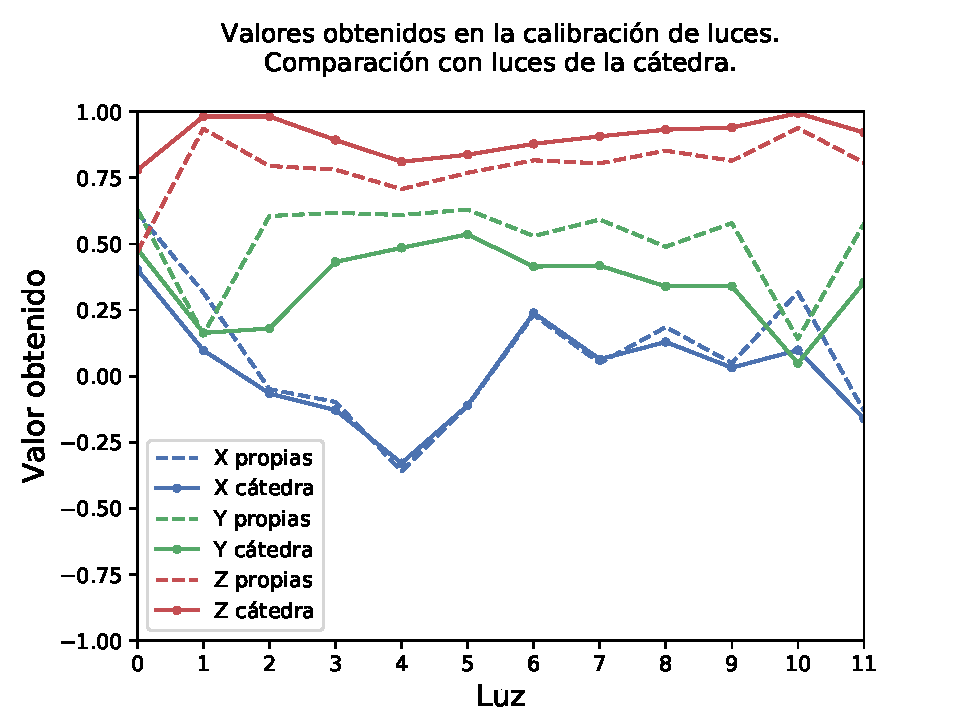
\includegraphics[scale=0.80]{informe/imagenes/lucesComparacionFinalMate.pdf}
    \captionof{figure}{Calibración de luces utilizando la esfera mate.}
    \end{figure}
}

Lo que observamos es que en líneas generales los valores nuestros y los de la cátedra dan parecidos, las curvas son similares. El eje X es el que más se aproxima al valor real, pero no sabemos por qué sucede esto sólo con este eje. Las diferencias que existen son de hasta 0.30 puntos (sobre 1.00), que si bien no parece demasiado, creemos que esto puede afectar el resultado final. \\

Veamos qué sucede si consideramos la esfera \textit{cromada}:

{\centering
\begin{figure}[H]
\centering
    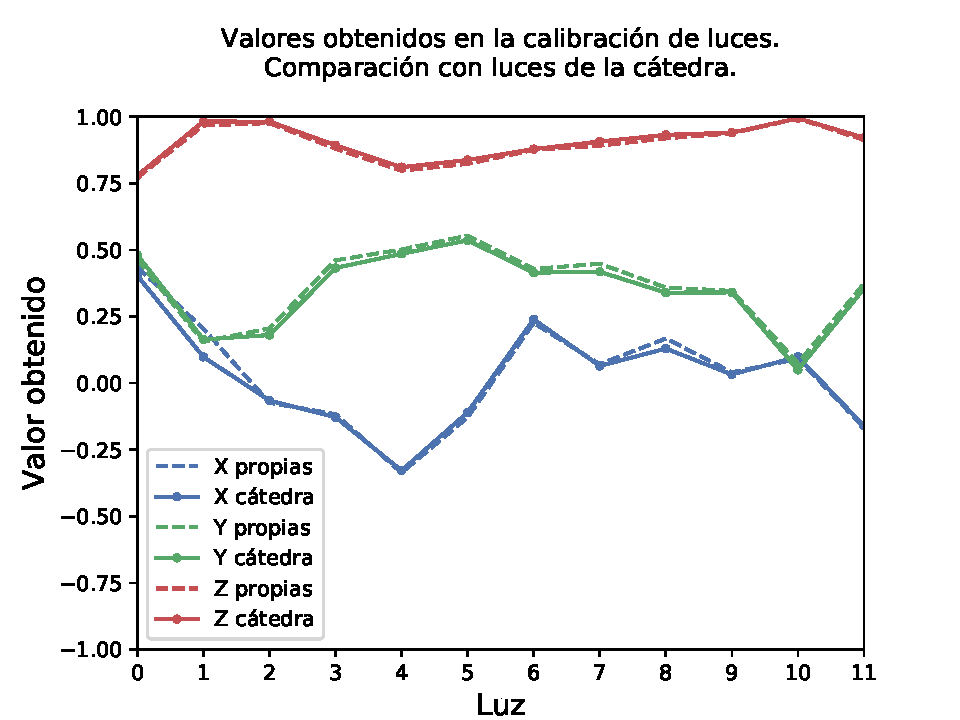
\includegraphics[scale=0.80]{informe/imagenes/lucesComparacionFinal.pdf}
    \captionof{figure}{Calibración de luces utilizando la esfera cromada.}
    \end{figure}
}

Para nuestra sorpresa, es claro que obtuvimos mejores resultados con la esfera cromada. Esperábamos obtener valores similares en ambas. Creemos que la razón por la que esto sucede, es porque en la esfera cromada es extremadamente notorio cuál es el punto mas brillante, por lo que es más exacta la identificación. En la esfera mate, en cambio, se tienen blancos muy similares en toda la imagen. \\

% 2. Como afecta la calibracion del sistema en el resto de las etapas \\
\newpage
\subsection{Normales}

En esta sección veremos cómo la calibración y elección de las luces afecta el resultado de las normales. En primer lugar, aprovecharemos que encontramos diferencias entre las luces obtenidas por la esfera mate y la esfera cromada para ver los errores que producen un set de luces 'desviado'. Por simplicidad, llamaremos a las luces de las tres categorías simplemente como: luces mate, cromadas y cátedra. \\

Sería muy razonable encontrarnos con algo de diferencia entre los sets de mate y cromada. Esperamos tambien que no haya diferencias entre cromada y cátedra, ya que los valores de luces eran prácticamente iguales. \\

En los gráficos que se encuentran a continuación, para cada píxel se grafica un vector que corresponde a la normal en ese punto. Como son \textit{miles} de normales, puede dar la impresión de que se grafican puntos pero no es así: son los vectores en forma de 'flechas'. Hay cientos de posibles combinaciones de luces a elegir, asi que sólo mostramos algunas. \\

{\centering
    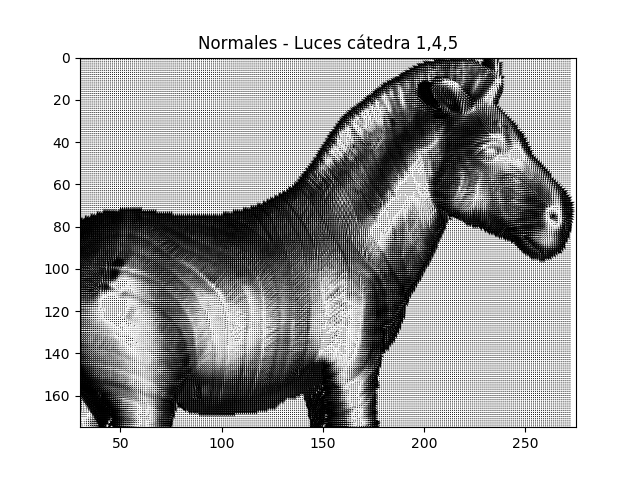
\includegraphics[scale=0.5]{informe/imagenes/normales/normalesLucesCatedra145.png}
    \captionof{figure}{Luces cátedra 1,4,5}
}

\begin{figure}[H]
\centering
\begin{minipage}{.5\textwidth}
  \centering
  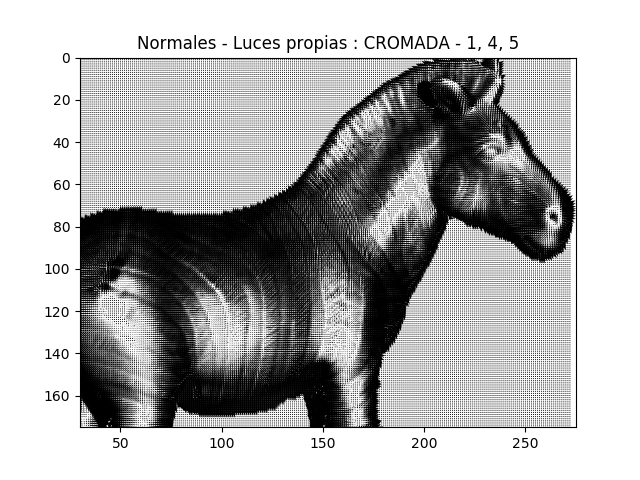
\includegraphics[width=1\linewidth]{informe/imagenes/normales/normalesLucesPropias145.png}
  \captionof{figure}{Luces cromadas 1,4,5}
  \label{fig:test1}
\end{minipage}%
\begin{minipage}{.5\textwidth}
  \centering
  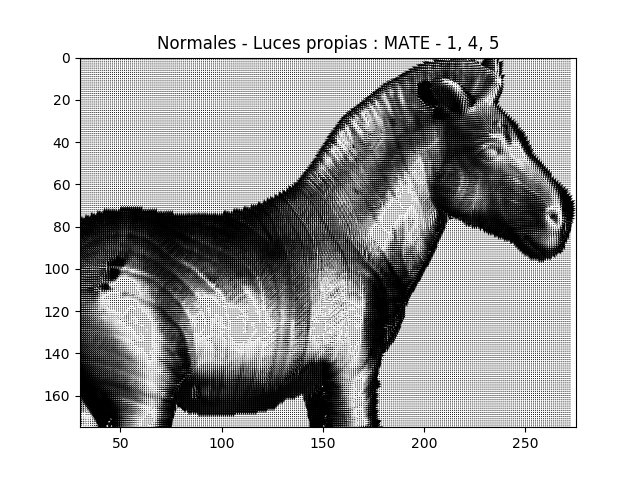
\includegraphics[width=1\linewidth]{informe/imagenes/normales/normalesLucesPropiasMate145.png}
  \captionof{figure}{Luces mate 1,4,5}
  \label{fig:test2}
\end{minipage}
\end{figure}

Con este set de luces podemos ver que no hay ninguna diferencia notable entre las normales producidas por el set de luces de la cátedra y el set de luces cromada. La mate es muy similar tambien, pero tiene zonas que son un poco mas claras, como por ejemplo en el rostro del caballo. De todos modos, las tres son similares entre sí. \\

% Este es medio similar creo que no vale la pena
% {\centering
%     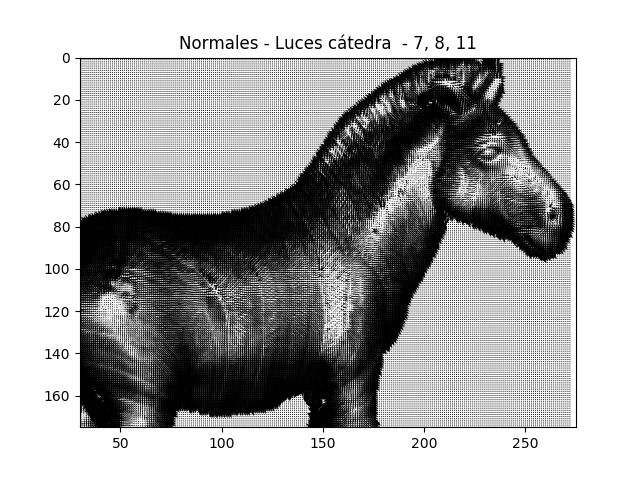
\includegraphics[scale=0.5]{informe/imagenes/normales/normalesLucesCatedra7811.png}
%     \captionof{figure}{Luces cátedra 7,8,11}
% }

% \begin{figure}[H]
% \centering
% \begin{minipage}{.5\textwidth}
%   \centering
%   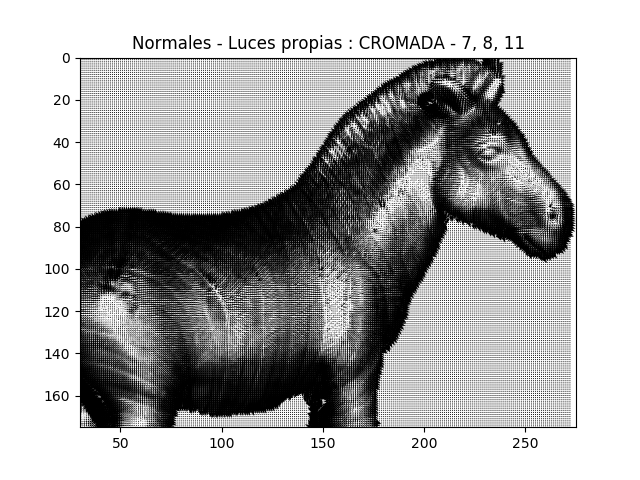
\includegraphics[width=1\linewidth]{informe/imagenes/normales/normalesLucesPropias7811.png}
%   \captionof{figure}{Luces cromadas 7,8,11}
%   \label{fig:test1}
% \end{minipage}%
% \begin{minipage}{.5\textwidth}
%   \centering
%   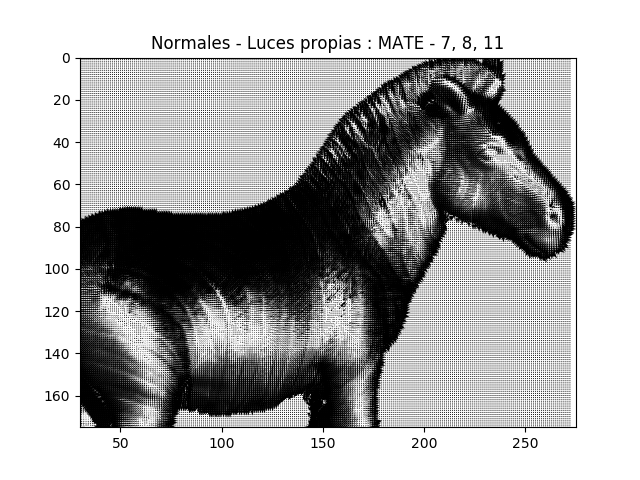
\includegraphics[width=1\linewidth]{informe/imagenes/normales/normalesLucesPropiasMate7811.png}
%   \captionof{figure}{Luces mate 7,8,11}
%   \label{fig:test2}
% \end{minipage}
% \end{figure}

En la mayoría de los sets que probamos obtuvimos resultados similares, con las luces cromada y cátedra obtenemos resultados casi idénticos y un poco de diferencia con el set mate. A continuación uno de los ejemplos un poco mas extremos que encontramos: \\

{\centering
    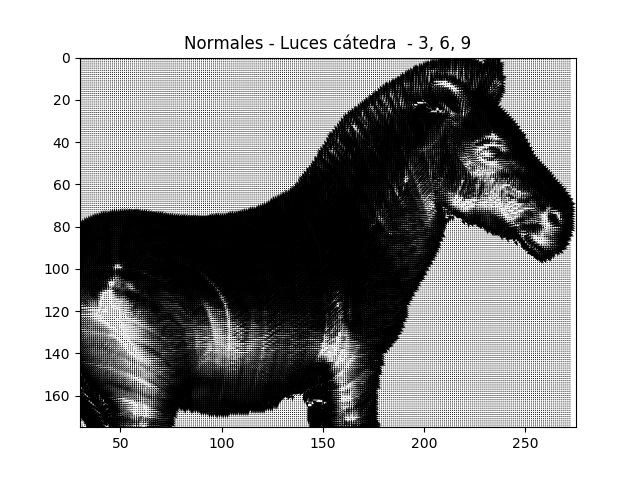
\includegraphics[scale=0.5]{informe/imagenes/normales/normalesLucesCatedra369.png}
    \captionof{figure}{Luces cátedra 3,6,9}
}

\begin{figure}[H]
\centering
\begin{minipage}{.5\textwidth}
  \centering
  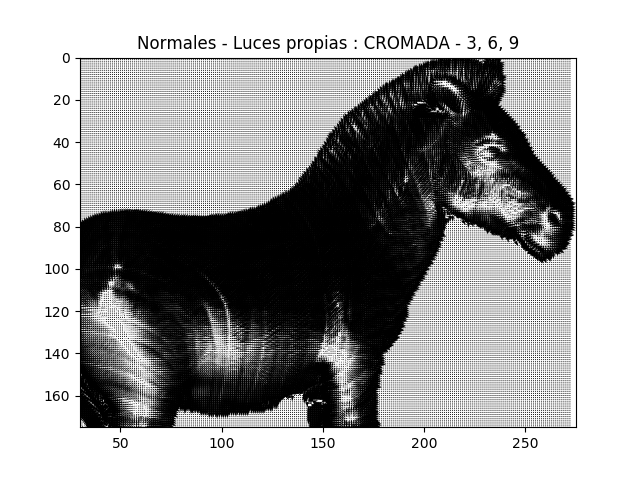
\includegraphics[width=1\linewidth]{informe/imagenes/normales/normalesLucesPropias369.png}
  \captionof{figure}{Luces cromadas 3,6,9}
\end{minipage}%
\begin{minipage}{.5\textwidth}
  \centering
  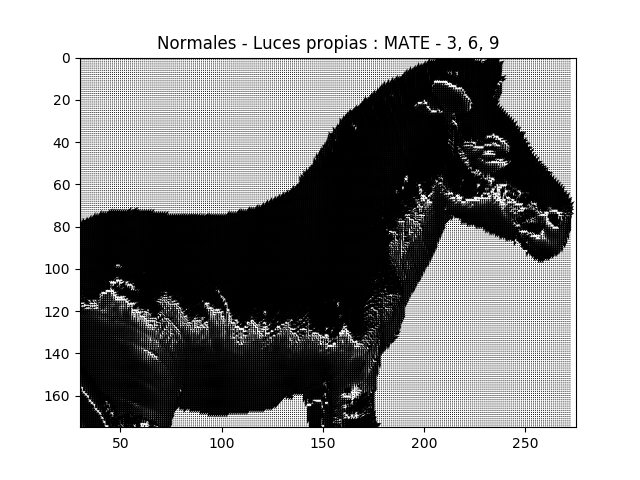
\includegraphics[width=1\linewidth]{informe/imagenes/normales/normalesLucesPropiasMate369.png}
  \captionof{figure}{Luces mate 3,6,9}
\end{minipage}
\end{figure}

En este caso es muy notoria la diferencia con el set mate. Esto muestra que no usar un set de luces correcto puede traer consecuencias notorias para el cálculo de las normales. Una calibración errónea acarrea errores notorios para el resto de las etapas. La similaritud entre los sets cromadas y cátedra se sigue mateniendo siempre, por lo que en los siguientes experimentos sólo consideraremos nuestro set de luces cromadas. \\

Lo siguiente que nos interesa ver es cómo afecta la elección de las tres luces en el cálculo de las normales. Para esto dejaremos fijas dos luces y moveremos una tercera. Elegimos para dejar fijas las luces 1 y 4 pues en las imágenes parecieran que apuntan en sentido inverso. \\

A continuación mostramos algunos de los resultados obtenidos, la mayoría se ven similares. \\

\begin{figure}[H]
\centering
\begin{minipage}{.5\textwidth}
  \centering
  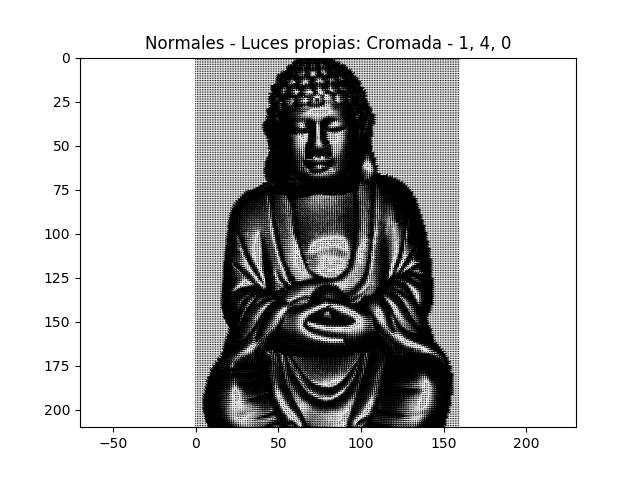
\includegraphics[width=1\linewidth]{informe/imagenes/normales/normalesBuda140.png}
  \captionof{figure}{$\uparrow$ Luces cromadas 1,4,0}
\end{minipage}%
\begin{minipage}{.5\textwidth}
  \centering
  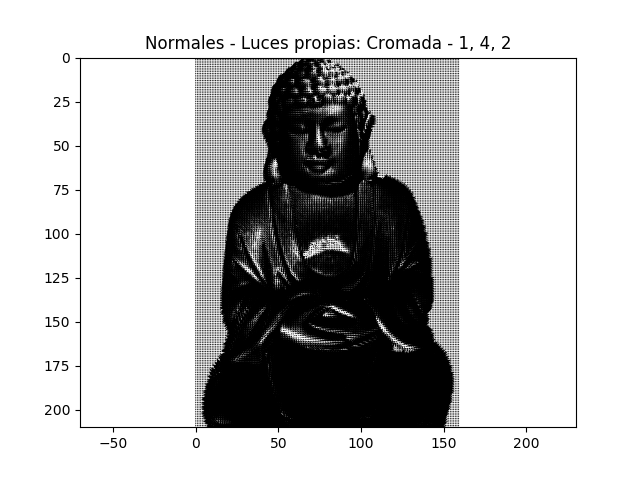
\includegraphics[width=1\linewidth]{informe/imagenes/normales/normalesBuda142.png}
  \captionof{figure}{$\uparrow$ Luces cromadas 1,4,2}
  \label{fig:normalesluz2}
\end{minipage}
\end{figure}

\begin{figure}[H]
\centering
\begin{minipage}{.5\textwidth}
  \centering
  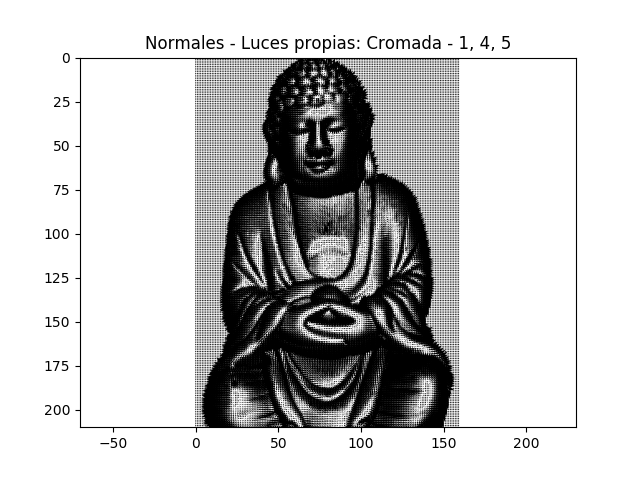
\includegraphics[width=1\linewidth]{informe/imagenes/normales/normalesBuda145.png}
  \captionof{figure}{$\uparrow$ Luces cromadas 1,4,5}
\end{minipage}%
\begin{minipage}{.5\textwidth}
  \centering
  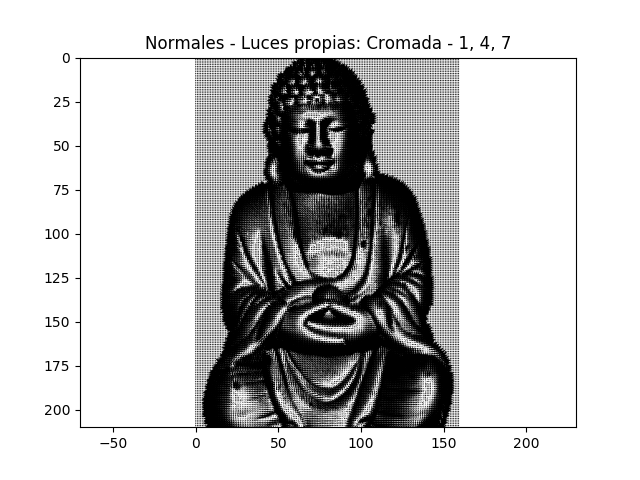
\includegraphics[width=1\linewidth]{informe/imagenes/normales/normalesBuda147.png}
  \captionof{figure}{$\uparrow$ Luces cromadas 1,4,7}
\end{minipage}
\end{figure}

\begin{figure}[H]
\centering
\begin{minipage}{.5\textwidth}
  \centering
  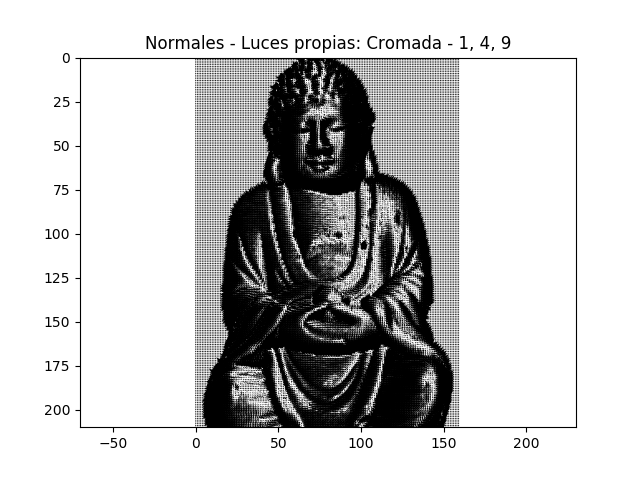
\includegraphics[width=1\linewidth]{informe/imagenes/normales/normalesBuda149.png}
  \captionof{figure}{$\uparrow$ Luces cromadas 1,4,9}
\end{minipage}%
\begin{minipage}{.5\textwidth}
  \centering
  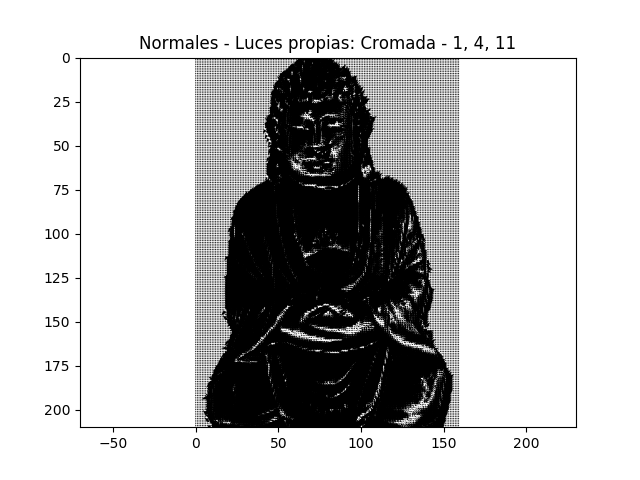
\includegraphics[width=1\linewidth]{informe/imagenes/normales/normalesBuda1411.png}
  \captionof{figure}{$\uparrow$ Luces cromadas 1,4,11}
  \label{fig:normalesluz11}
\end{minipage}
\end{figure}

En la mayoría de los casos se obtuvieron resultados similares. Las excepciones se ven en la \textit{Figura \ref{fig:normalesluz2}} y la \textit{Figura \ref{fig:normalesluz11}} dónda la tercera luz es la 2 y la 11 respectivamente. Observando las imágenes reales, la imagen con luz 11 es muy similar a la que tiene luz 4, mientras que la imagen con luz 2 es similar a la de luz 1. Para el resto de las imágenes hay diferencias más notorias entre los ángulos de luz. Esto último nos da la pauta de que se obtienen mejores resultados si los ángulos de luces son mas variados.

















\newpage
\subsection{Profundidades}

En esta sección analizaremos los resultados finales de la aplicación del método. Más precisamente, analizaremos las profundidades que obtuvimos siguiendo el proceso descripto en la sección desarrolo, utilizando nuestras luces de calibración (que resultaron casi idénticas a las de la cátedra). \\

En primer lugar queremos darnos una idea general de qué tan correctos son nuestros valores. Para esto tomaremos las profundidades obtenidas y graficaremos las curvas de nivel, marcando con diferentes colores cada capa de profundidades. \\


% \todo[inline]{Graficos curvas de nivel}

% {\centering
%     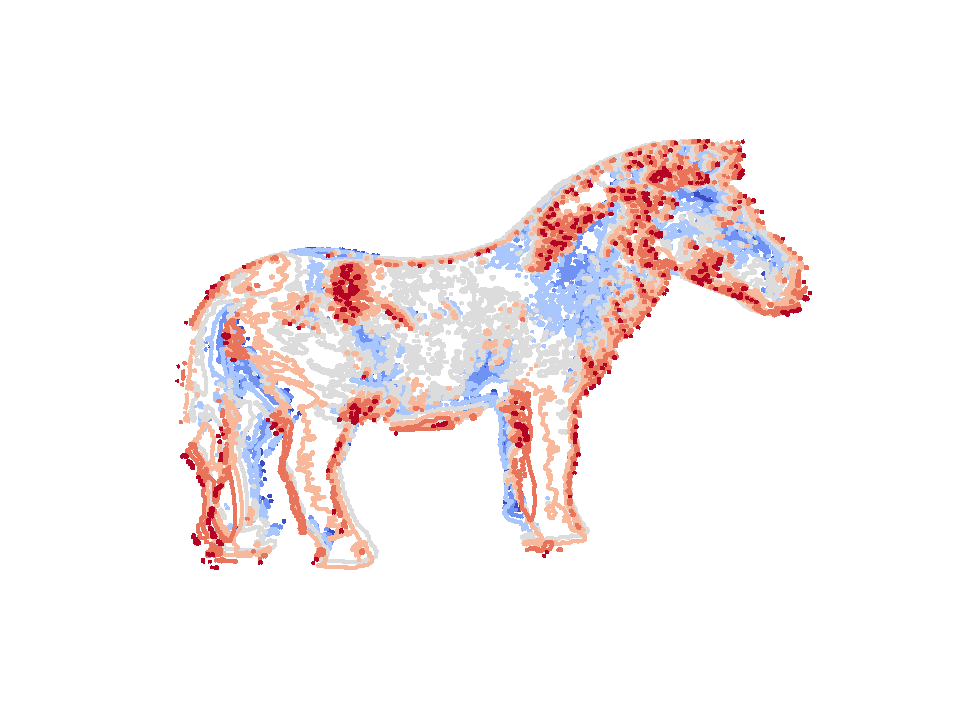
\includegraphics[scale=0.6]{informe/imagenes/supnivel/supNivelCaballoLucesPropias578N1.pdf} \\
% }
% {\centering
%     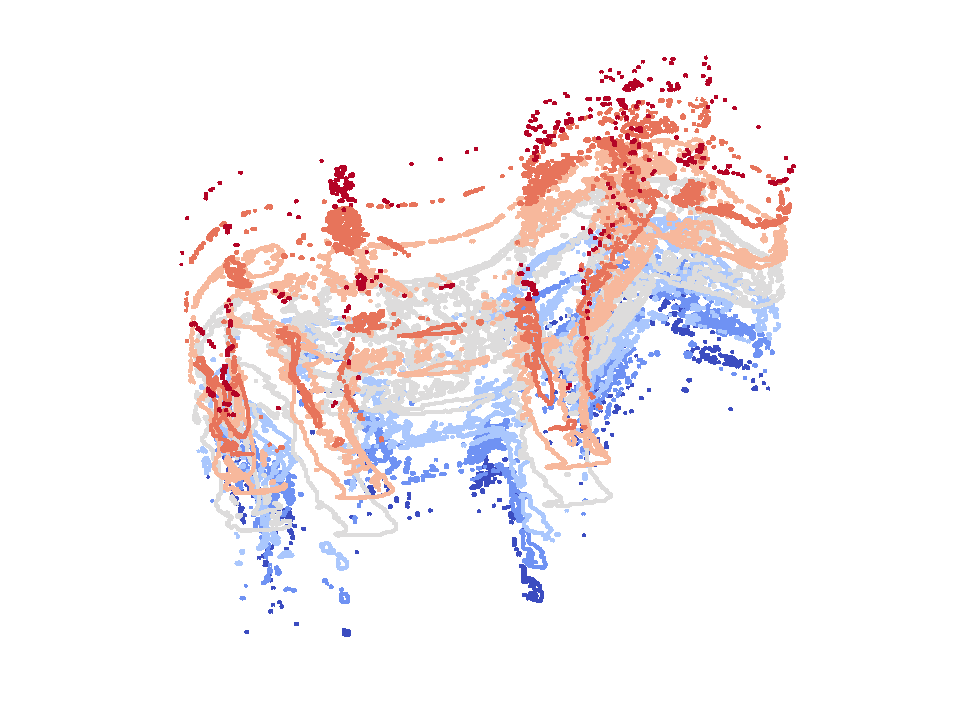
\includegraphics[scale=0.6]{informe/imagenes/supnivel/supNivelCaballoLucesPropias578N2.pdf} \\
% }
% {\centering
%     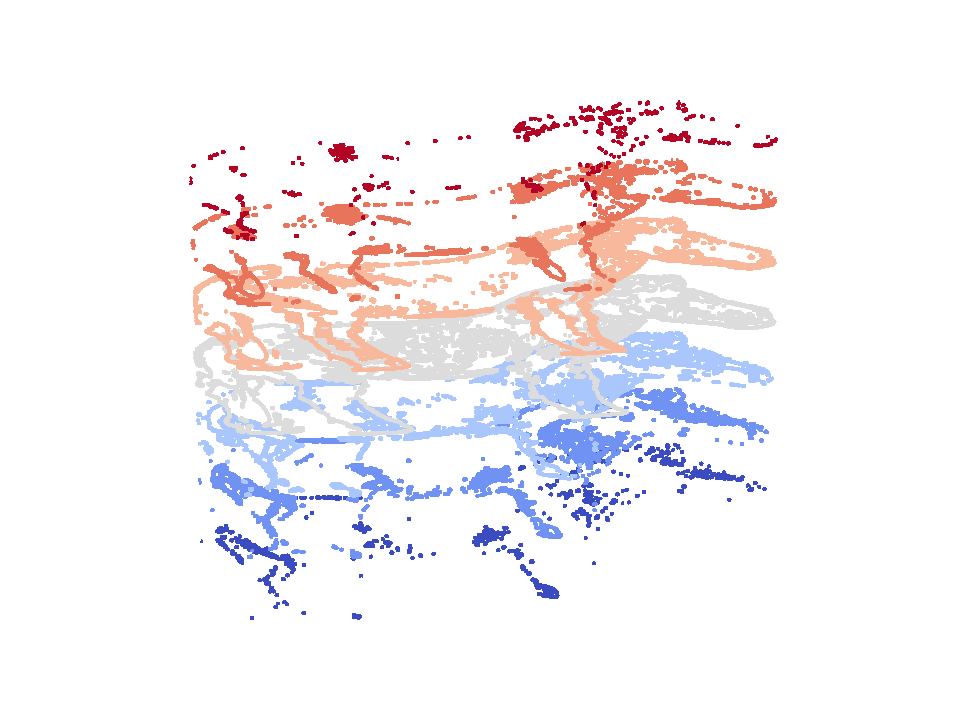
\includegraphics[scale=0.6]{informe/imagenes/supnivel/supNivelCaballoLucesPropias578N3.pdf}
%     \captionof{figure}{\textit{Curvas de nivel de la función de profundidad (para cada píxel, su profundidad estimada) Los valores fueron calculados utilizando las luces que obtuvimos en nuestra calibración.}}
% }

{\centering
    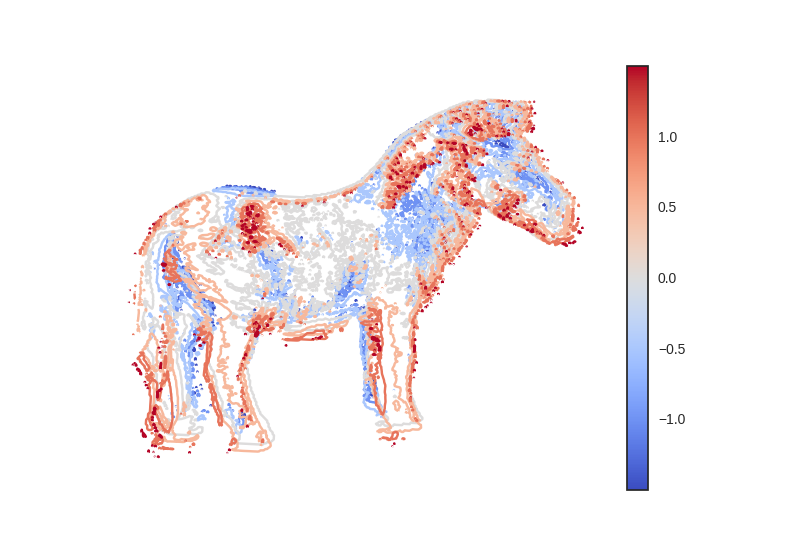
\includegraphics[width=0.80\linewidth]{informe/imagenes/supnivel/supNivelCaballoLucesPropias578N1.png}
    \captionof{figure}{Superficies de nivel, vista superior}
}

{\centering
    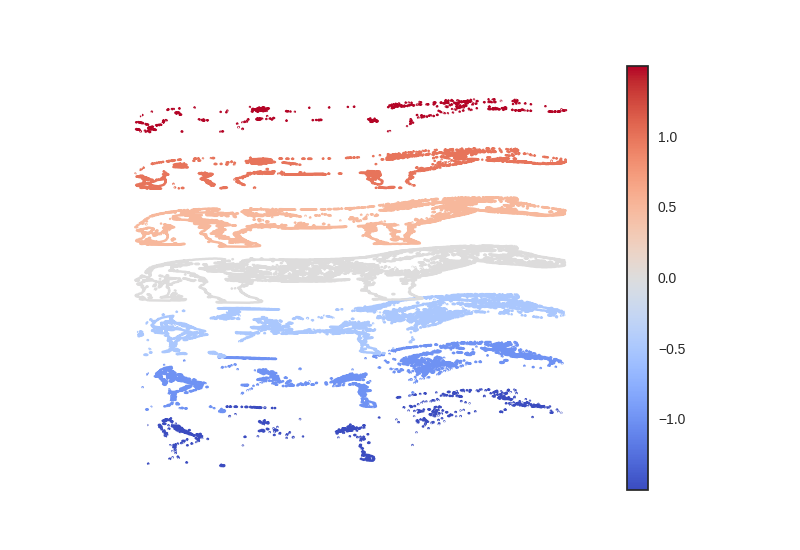
\includegraphics[width=0.80\linewidth]{informe/imagenes/supnivel/supNivelCaballoLucesPropias578N3.png}
    \captionof{figure}{Superficies de nivel, vista lateral\\}
}

$ $\newline
Con esto podemos ver que las profundidades son adecuadas y la figura original del caballo es distinguible. Notamos que en los bordes de la imagen hay gran cantidad de rojos: creemos tiene que ver con que al haber usado la máscara, la diferencia de alturas es muy brusca entre la figura y el plano del fondo.  \\

Si consideramos la superficie completa de profundidad en un modelo 3D, los resultados no fueron perfectos tampoco. Los sets de luces utilizados fueron elegidos arbitrariamente. \\

{\centering
    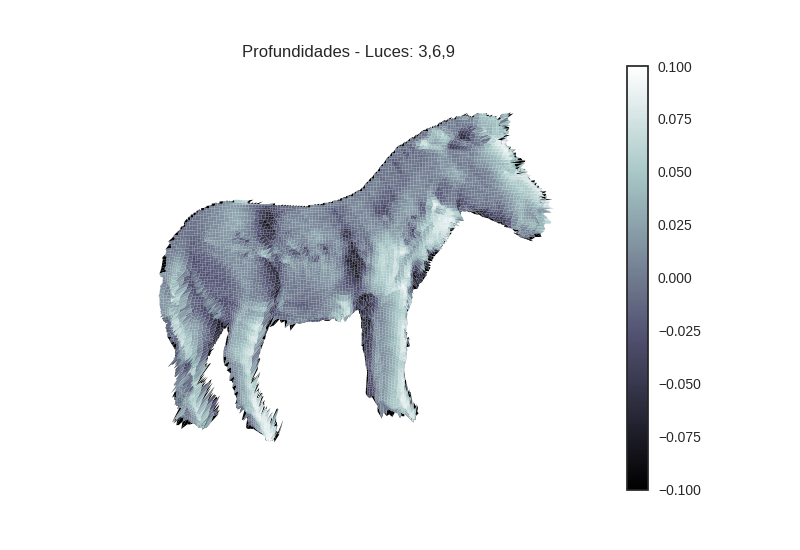
\includegraphics[width=0.80\linewidth]{informe/imagenes/profundidades/profsCaballo369.png}
    \captionof{figure}{Profundidades utilizando luces 3,6,9}
}

$ $\newline
Aquí podemos ver como la forma general se distingue bastante bien, y que las zonas mas iluminadas del modelo se corresponden con las zonas iluminadas de las imágenes originales. Sin embargo, hay muy pocos detalles presentes, sobre todo en el rostro del caballo. Es posible que el problema sea la elección de las luces, pero no es el caso, pues se obtienen modelos similares también con otras elecciones: \\

{\centering
    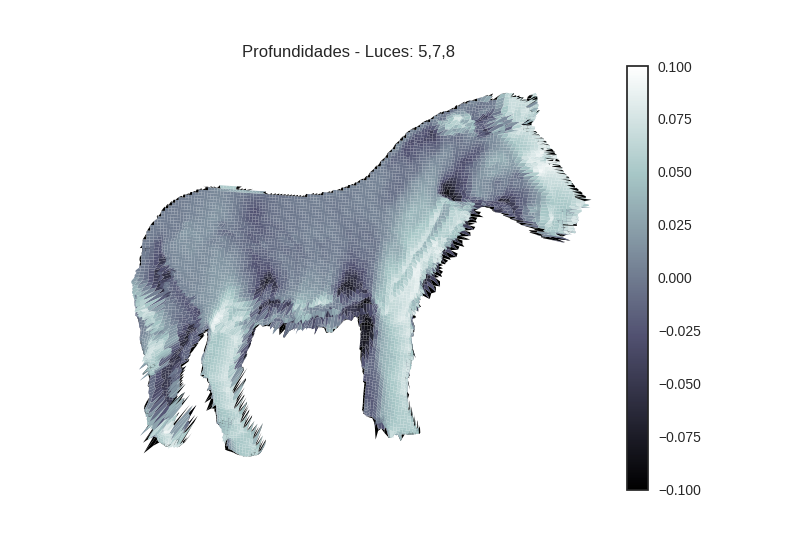
\includegraphics[width=0.80\linewidth]{informe/imagenes/profundidades/profsCaballo578.png}
    \captionof{figure}{Profundidades utilizando luces 5,7,8}
}

\todo[inline]{Probar algunas combinaciones mas pues probablemente haya alguna mejor}


$ $\newline
Aunque las profundidades son distinguibles en los casos que mostramos, los resultados no son lo que esperábamos. Los modelos obtenidos no se corresponden con el modelo propuesto en el enunciado. Podemos ver que nuestro modelo esta lleno de picos, sobre todo en el borde de la figura. Creemos que los resultados tienen que ver con una combinación de errores numéricos y los cálculos de los planos tangentes, no pudimos detectar una falla específica y obtener resultados mejores. Aún así, consideramos que lo que obtuvimos son resultados razonables. \\

% En la imagen de arriba podemos ver lo que mencionamos sobre la \textit{suavidad} de la superficie. Es claro que es diferente a lo visto en la imagen de ejemplo del enunciado, pero incluso así son distinguibles las alturas de los diferentes píxeles. El \textit{fondo} del modelo es un plano perfecto por el hecho de haber utilizado la máscara para no realizar cálculos innecesarios. Sospechamos que los picos tiene que ver con la forma en que aproximamos los planos tangentes. Veamos que obtenemos si partimos directamente de las \textbf{normales} provistas por la cátedra:

% {\centering
%     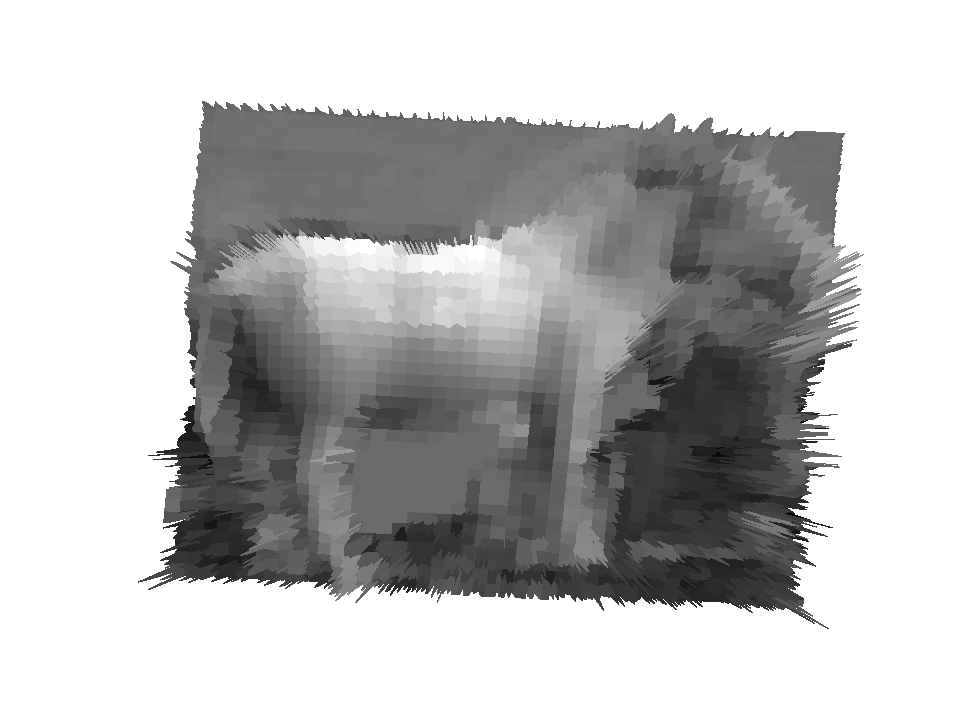
\includegraphics[scale=0.65]{informe/imagenes/profundidadesCaballoNormalescatedra.pdf} \\
% }

% Si bien las luces con las que fueron obtenidas las normales de la cátedra son desconocidas para nosotros, podemos hacer algunas comparaciones. Aunque esté llena de \textit{picos}, sobretodo en los bordes, parece ser una superficie un poco más suave que la obtenida por nosotros. Dado que no sabemos cuáles fueron las luces utilizadas en el cálculo, no podemos descartar que sea un tema de elección de luces. Sin embargo, incluso aunque fuesen las mismas, veremos más adelante que lo calibrado por nosotros no se corresponde en un 100\% por lo que es esperable que se observen diferencias. \\

Otra cosa clara es que los detalles (por ejemplo el rostro) se pierden. Si bien era esperable ya que son áreas delicadas, nos da la pauta de que nuestras aproximaciones parecen no ser del todo correctas. De todos modos, no podemos saber si en una estimación 'bien hecha' los detalles se mantienen o no. \\


En los resultados que presentamos utilizamos el promedio de los colores para obtener los datos de la imagen origial. Veremos qué sucede si en vez del promedio consideramos las diferentes componenetes de color por separado. No esperamos obtener diferencias significativas entre tomar el promedio o una sola componente del color.

\todo[inline]{Profundidades de caballo mismo set de luces, diferentes tomadas de colores}


% {\centering
%     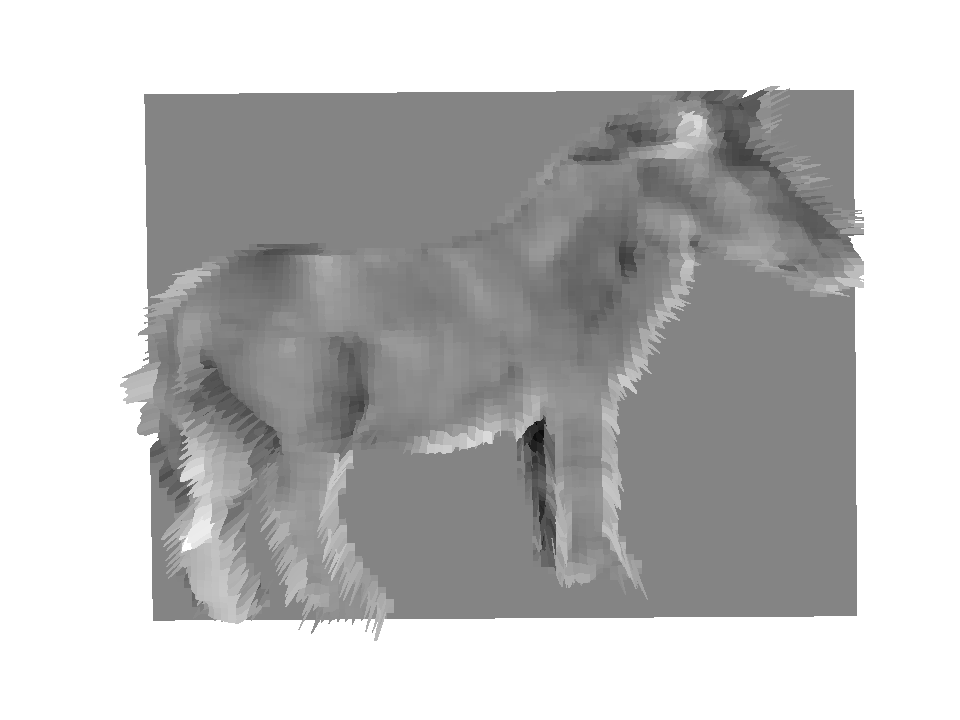
\includegraphics[scale=0.5]{informe/imagenes/profundidades/profCaballo012ColorProm.pdf}
%     \captionof{figure}{$\uparrow$ Luces 0,1,2, promedio de colores}
%     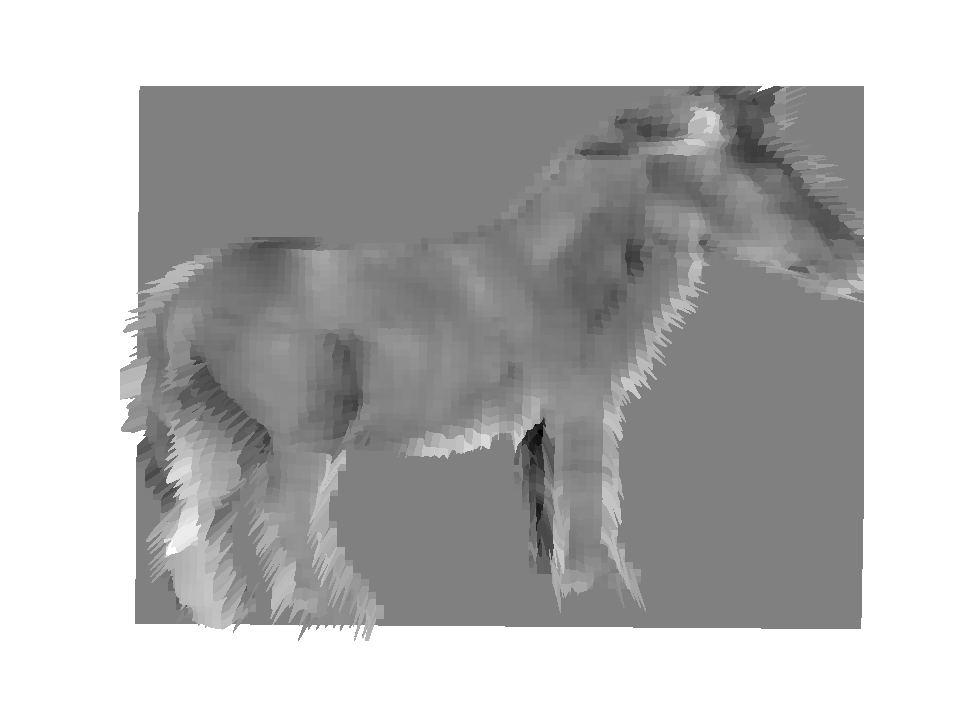
\includegraphics[scale=0.49]{informe/imagenes/profundidades/profCaballo012ColorAzul.pdf}
%     % \captionof{figure}{\textit{Luces 0,1,2, componente azul}}
%     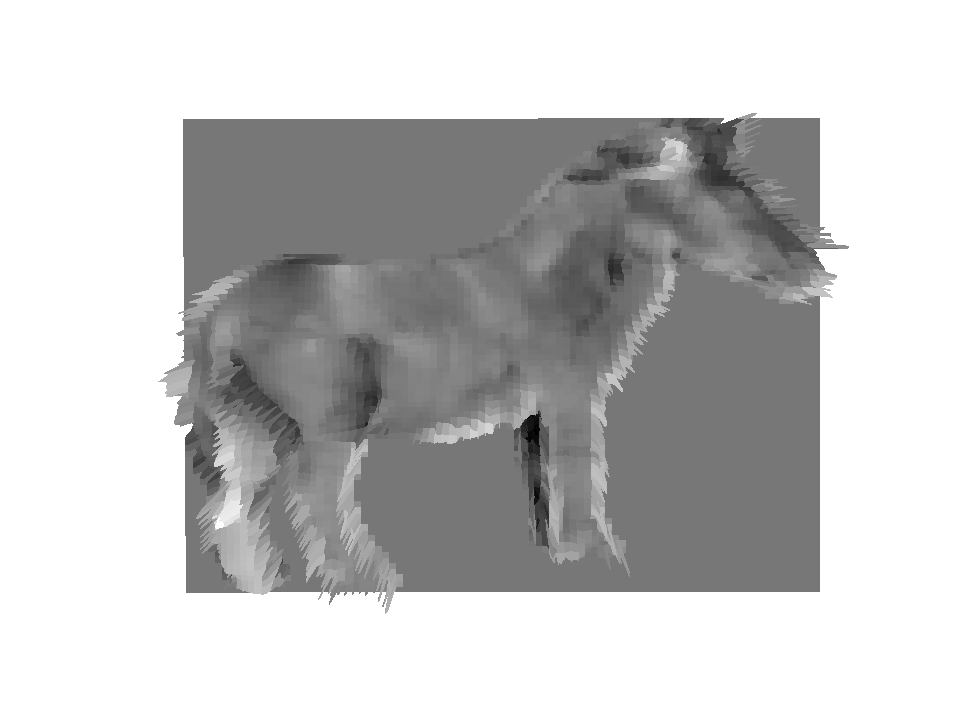
\includegraphics[scale=0.54]{informe/imagenes/profundidades/profCaballo012ColorRojo.pdf}
%     % \captionof{figure}{\textit{Luces 0,1,2, componente roja}}
% }
% \begin{center}
%     Luces 0,1,2, componente azul (izq), componente roja (der)
% \end{center}

Cómo sospechabamos, no hay ninguna diferencia apreciable en tomar las imágenes con diferentes componentes de color. Pensamos que una posibilidad es que la nula diferencia se deba al color del objeto original. Tomemos entonces una imagen con colores, como es el caso del gato. Creemos que seguirá sin haber diferencias apreciables, pues el promedio de los colores de cierta forma engloba a todos los datos. \\


\begin{figure}[H]
\centering
\begin{minipage}{.5\textwidth}
  \centering
  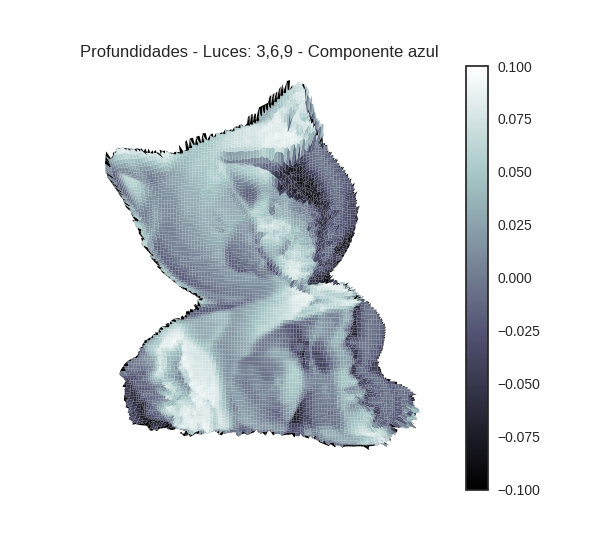
\includegraphics[width=1\linewidth]{informe/imagenes/profundidades/gato369Azul.png}
  \captionof{figure}{Luces 3,6,9 - Componente Azul}
\end{minipage}%
\begin{minipage}{.5\textwidth}
  \centering
    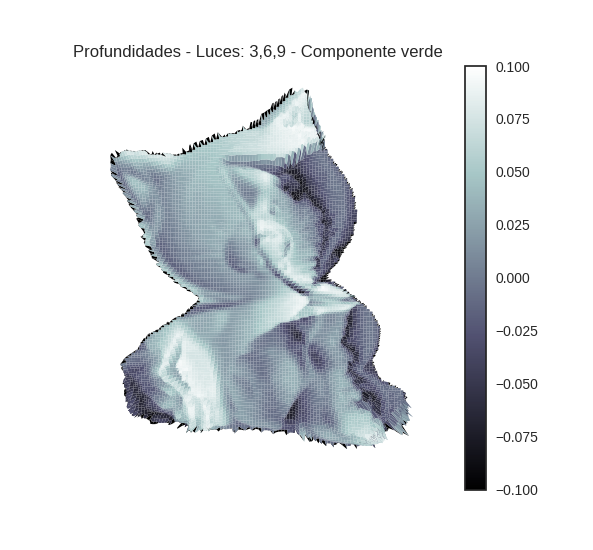
\includegraphics[width=1\linewidth]{informe/imagenes/profundidades/gato369Verde.png}
    \captionof{figure}{Luces 3,6,9 - Componente Verde}
\end{minipage}
\end{figure}

{\centering
  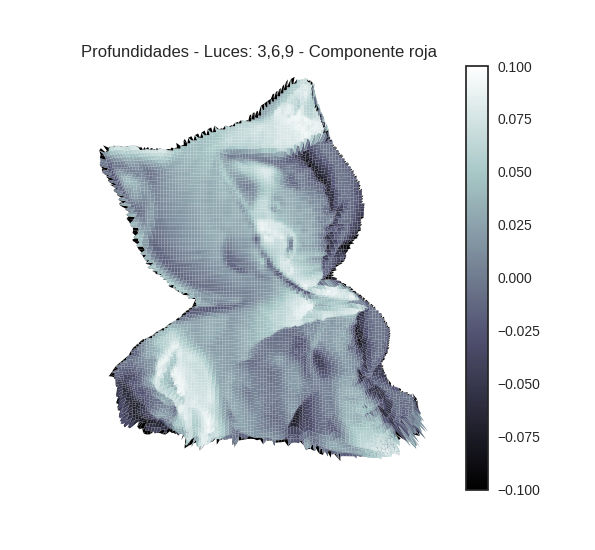
\includegraphics[width=0.5\linewidth]{informe/imagenes/profundidades/gato369Rojo.png}
  \captionof{figure}{Luces 3,6,9 - Componente Roja}
}

$ $\newline
Las tres componentes se ven bastante similares, aunque hay algunas diferencias. La componente azul es la que parece tener los detalles más marcados, ver por ejemplo en los ojos del gato. La componente roja tiene menos detalles y en todo el modelo se vé de un color más claro que los demás, es decir la profundidad obtenida es un poco diferente. Entonces en una imagen en color, contrario a lo que sucede con una imagen blanco y negro, las diferentes componentes de color tienen inferencia en el resultado final, aunque no demasiada. \\

Más allá de las diferencias entre componentes, es claro que en la figura del gato hay una sombra muy extraña en la mitad derecha del rostro, que parece ser muy similar al contorno de una oreja izquierda. Para descartar que sea problemas con el set de luces elegido, repetimos el mismo experimento con un set de luces diferentes. Aprovechamos además para ver si los colores influyes de diferente manera con otro set. \\

\begin{figure}[H]
\centering
\begin{minipage}{.5\textwidth}
  \centering
  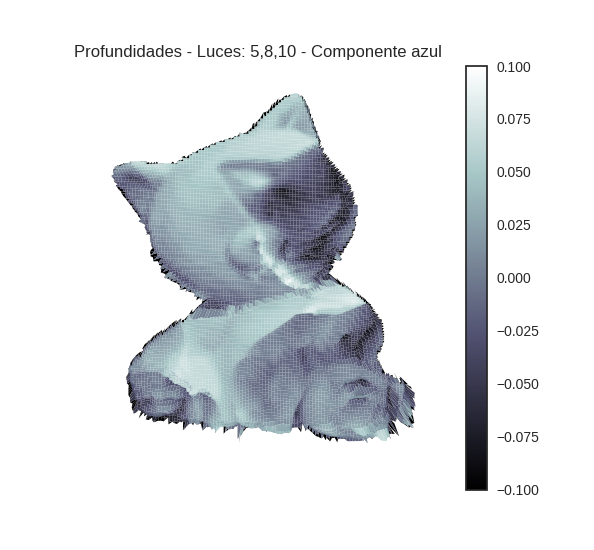
\includegraphics[width=1\linewidth]{informe/imagenes/profundidades/gato5810Azul.png}
  \captionof{figure}{Luces 5,8,10 - Componente Azul}
\end{minipage}%
\begin{minipage}{.5\textwidth}
  \centering
    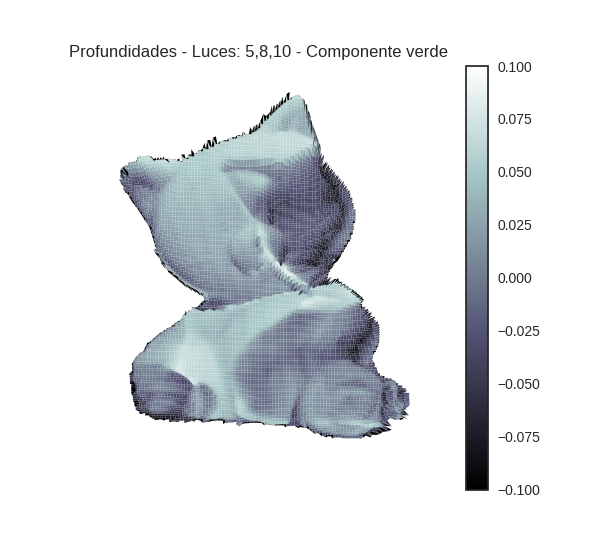
\includegraphics[width=1\linewidth]{informe/imagenes/profundidades/gato5810Verde.png}
    \captionof{figure}{Luces 5,8,10 - Componente Verde}
\end{minipage}
\end{figure}

{\centering
  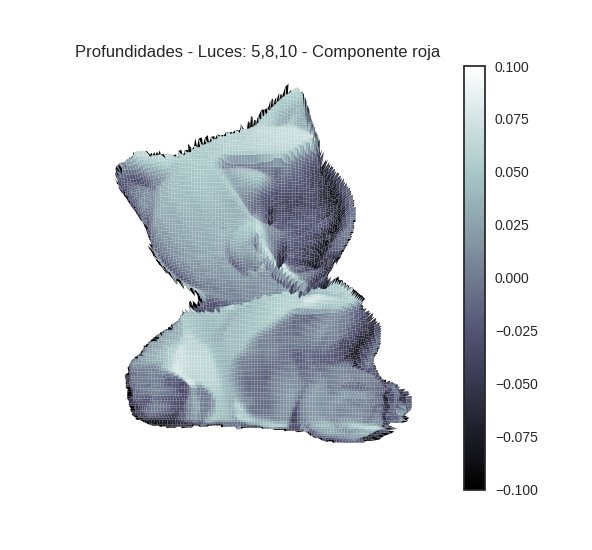
\includegraphics[width=0.5\linewidth]{informe/imagenes/profundidades/gato5810Rojo.png}
  \captionof{figure}{Luces 5,8,10 - Componente Roja}
}

$ $\newline
En las últimas tres figuras utilizamos un set diferente pero tenemos un comportamiento similar al de antes: la componente azul maneja una cantidad de detalles un poco mayor que las demás, notorios en la parte inferior de la figura. Sin embargo con este set de luces la diferencias entre las componentes son mucho menores. Además, seguimos observando la sombra extraña en el lado derecho del rostro, que ahora estamos bastante seguros que es algún problema con nuestro sistema. Lamentablemete no pudimos hallar su causa para solucionarlo y obtener mejores resultados. \\

Es interesante notar que en los ejemplos anteriores utilizamos diferentes combinaciones de luces y obtuvimos profundidades diferentes (pero similares) entre los sets. En el ejemplo del gato, con el primer set de luces logramos conseguir más detalles que con el segundo set, pero pensábamos que las diferencias iban a ser más contundentes. En el siguiente experimento intentaremos ver cómo la elección de luces repercute en las profundidades finales. Para ello, realizamos los cálculos de profundidad con una imagen que tiene más detalles. \\

Los siguientes son gráficos con las profundidades de Buda, fijando las dos primeras luces y haciendo variar una tercera, al igual que hicimos con el experimento de las normas en la sección anterior. \\

\begin{figure}[H]
\centering
\begin{minipage}{.5\textwidth}
  \centering
  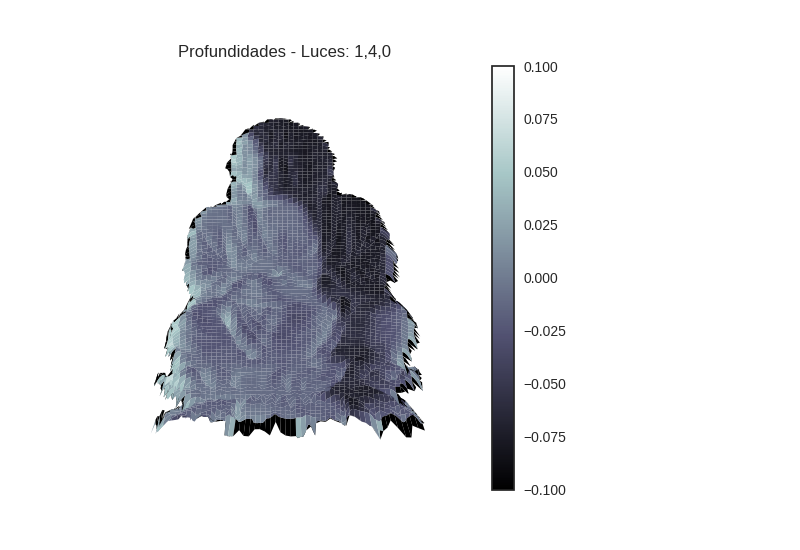
\includegraphics[width=1.3\linewidth]{informe/imagenes/profundidades/buda140.png}
  \captionof{figure}{Profundidades - Luces 1,4,0}
\end{minipage}%
\begin{minipage}{.5\textwidth}
  \centering
    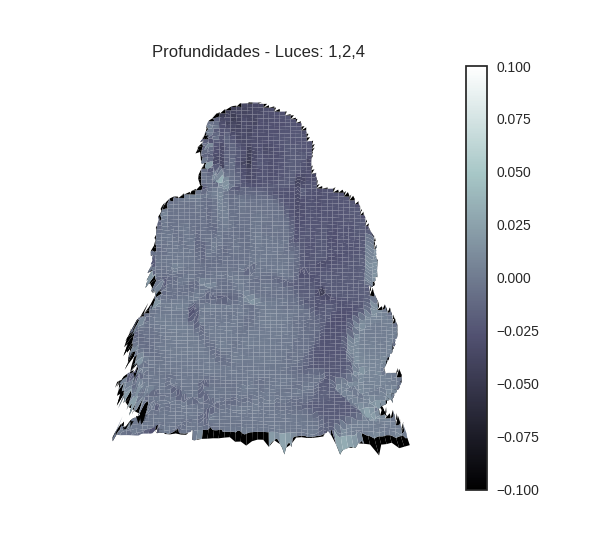
\includegraphics[width=1.3\linewidth]{informe/imagenes/profundidades/buda142.png}
  \captionof{figure}{Profundidades - Luces 1,4,2}
\end{minipage}
\end{figure}


\begin{figure}[H]
\centering
\begin{minipage}{.5\textwidth}
  \centering
  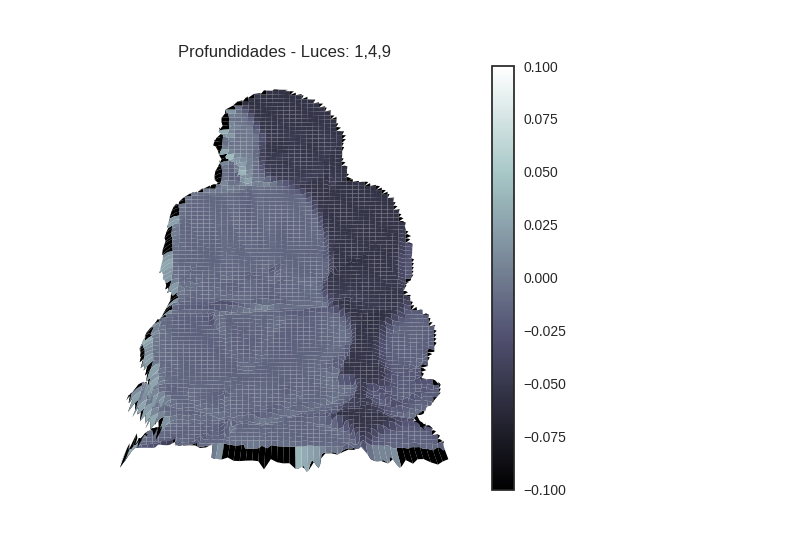
\includegraphics[width=1.3\linewidth]{informe/imagenes/profundidades/buda149.png}
  \captionof{figure}{Profundidades - Luces 1,4,9}
\end{minipage}%
\begin{minipage}{.5\textwidth}
  \centering
    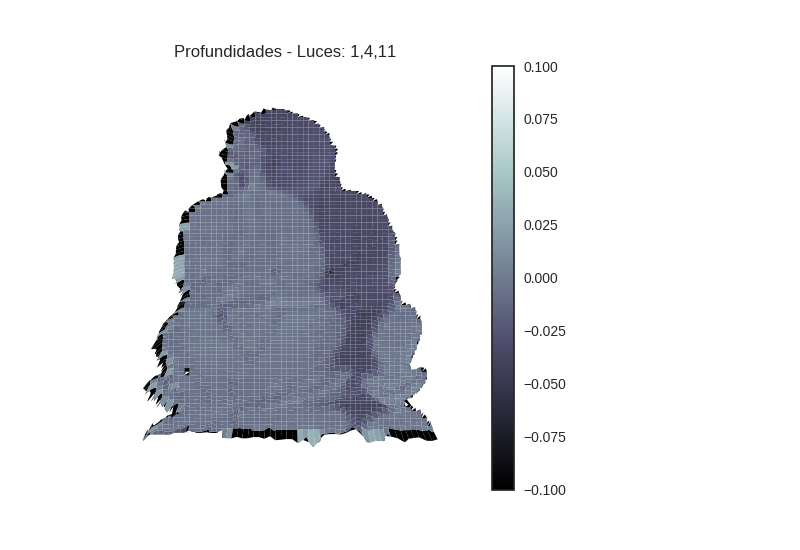
\includegraphics[width=1.3\linewidth]{informe/imagenes/profundidades/buda1411.png}
  \captionof{figure}{Profundidades - Luces 1,4,11}
\end{minipage}
\end{figure}


\todo[inline]{CONCLUIR ALGO SOBRE LOS GRAFICOS DE BUDA}


\newpage
\subsection{Eliminacion gaussiana y Factorización LU}

Lo que queremos lograr con esta experimentación es comparar el resultado del cálculo sobre todos los píxeles usando el método de eliminación gaussiana vs factorizar la matriz y resolver los dos sistemas triangulados.
Para esto tomamos una matriz cualquiera de las generadas por 3 luces y resolvimos el sistema para N términos independientes distintos generados al azar. Esto simula el correr el algoritmo sobre una imagen de N píxeles.\\

Medimos únicamente el tiempo que tarda en resolver el sistema para cada píxel, dejando de lado todo cálculo extra por afuera de la medición (como por ejemplo la generacion aleatoria de los términos independientes). Luego sumamos cada uno de estos tiempos como la medición del experimento de tamaño N.
Hicimos 100 mediciones para cada cantidad de píxeles y luego dividimos por esa cantidad para sacar el promedio, de esta manera reducimos el ruido que pudo haberse visto durante la medición.

Hicimos varias mediciones variando la cantidad de píxeles y estos fueron los resultados:

{\centering
    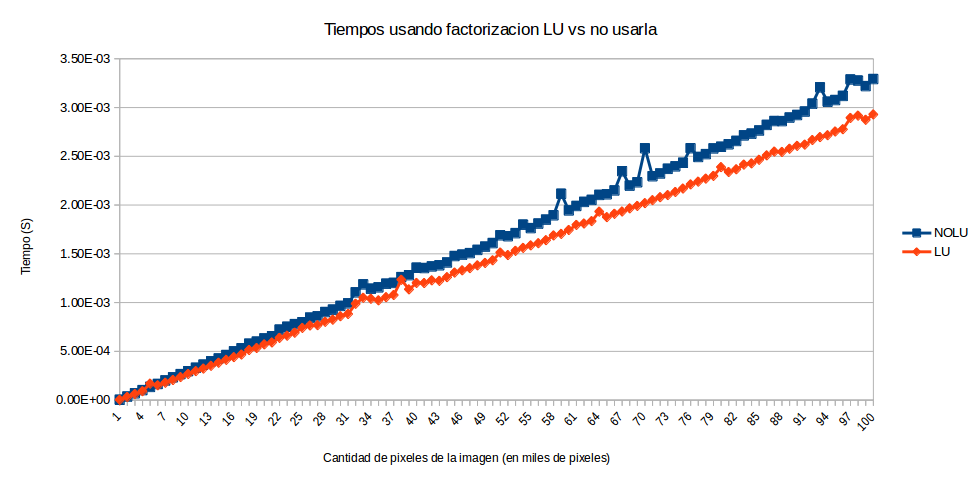
\includegraphics[scale=0.7]{informe/imagenes/LUVSNOLU.PNG} \\
}

Como vemos ambos casos están en funcion lineal con la cantidad de píxeles, esto es gracias a que, aunque resolver un sistema sea cuadrático y el otro cúbico, ambos están resolviendo sistemas de 3x3 N veces, por lo tanto el tiempo que tarda en resolver un sistrema u otro se vuelve una constante que multiplica a N y por lo tanto tenemos órdenes lineales para los dos casos.\\

Es por esto que quisimos hacer otro experimento más para comparar la diferencia entre el tiempo cuadrático de resolver el sistema ya factorizado y de resolver el sistema utilizando eliminación gaussiana.
Para esto creamos instancias de matrices cada vez más grandes y las duplicamos, a una le aplicamos eliminación gaussiana y a la otra la factorizamos y luego resolvimos los dos sistemas (L y U). Es importante destacar que no tomamos el tiempo que toma la factorizacion ya que este es un tiempo que se amortiza en la cantidad de operaciones y no era lo que queríamos comprobar.

El resultado fue el siguiente:

{\centering
    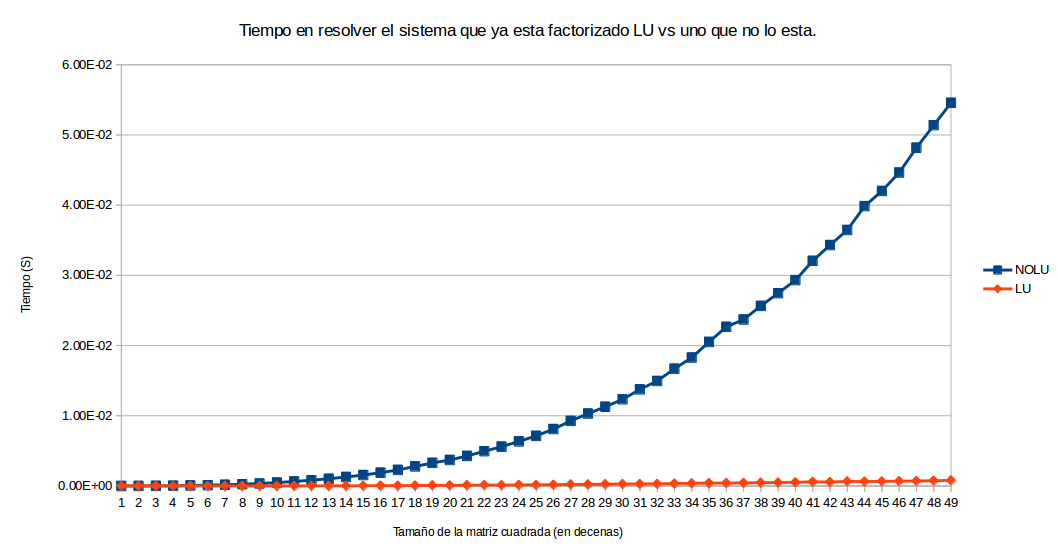
\includegraphics[scale=0.6]{informe/imagenes/LUVSNOLUDIM.PNG} \\
}

Dado que los tiempos para la medición de LU son muy pequeños, decidimos hacer otro gráfico con escala logarítmica para apreciar mejor la diferencia.


{\centering
    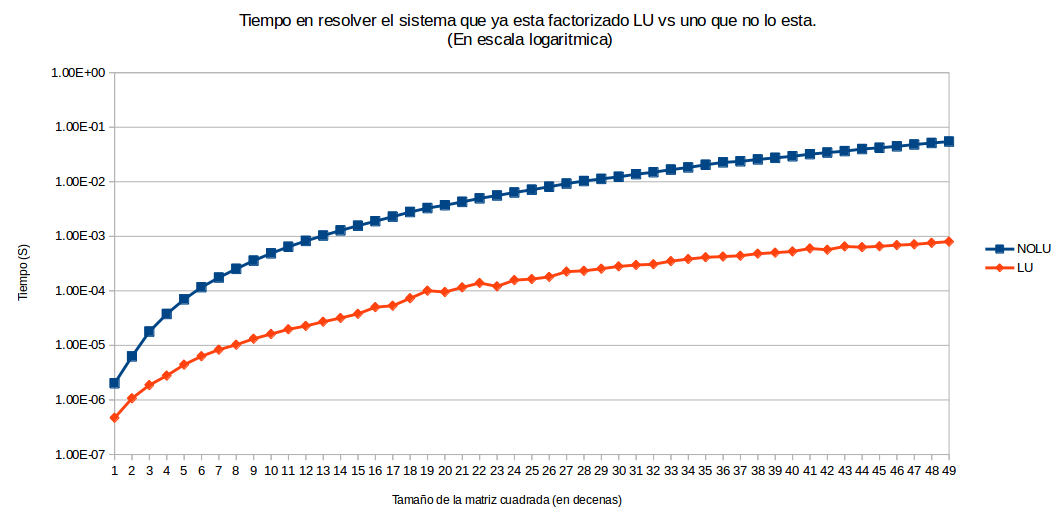
\includegraphics[scale=0.6]{informe/imagenes/LUVSNOLUDIMLOG.PNG} \\
}

Como podemos ver, efectivamente hay un crecimiento polinomial de ambos y la factorizacion LU crece en menor magnitud con el tamaño del sistema a resolver.

\subsection{Cholesky}

A continuación presentamos un análisis temporal de los métodos utilizados comparados con Cholesky. Para realizar estos análisis y poder hacer compararciones con la eliminació gaussiana y LU, generamos matrices que todos los métodos pueden resolver. Creamos de forma automatizada matrices simétricas definidas positivas, generando matrices $A$ con coeficientes aleatorios de 0 a 1 de tamaño $n$ y las multiplicamos por su traspuesta $A^{t}$. Luego les sumamos el valor $n$ en la diagonal garantizando que sean diagonal dominante y se las multiplica por un escalar para evitar valores muy cercanos al 0 que podrían ser inconvenientes para los métodos menos estables. \\

% En estos experimentos intentamos corroborar la complejidad asintótica de los métodos, generando matrices de dimensiones crecientes que resolvimos iterativamente por cada método, promediando el tiempo de ejecución para cada tamaño de matriz. En las mediciones no consideramos lo tiempos de creación de matrices y/o descomposición, sino que únicamente el tiempo de resolución. \\

Una de las ventajas más importantes de las descomposiciones utilizadas es la de no tener que recalcular la matriz a resolver en cada iteración realizada si sólo se cambia el término independiente. Para observar este comportamiento utilizamos matrices de dimensión $500*500$ y resolvimos el sistema $Ax = b$ varias veces midiendo el tiempo que se tomaba en resolver el mismo. \\

Lo esperado es que Gauss sea el método más lento en este tipo de pruebas, ya que debe re-triangular la matriz cada vez que quiere resolver para un nuevo $b$. En cambio, Cholesky y LU una vez que su descomposición es encontrada, sólo deben realizarse despejes. Sobre el eje $x$ puede verse la \textit{cantidad acumulada} de términos independientes, y en el eje $y$ el tiempo en segundos. \\
% Por un lado simplemente medimos el tiempo total que tardaba cada iteracion de resolucion y por el otro sumamos los tiempos tomados en resolver todos los sistemas anteriores.
\hspace*{-2cm} 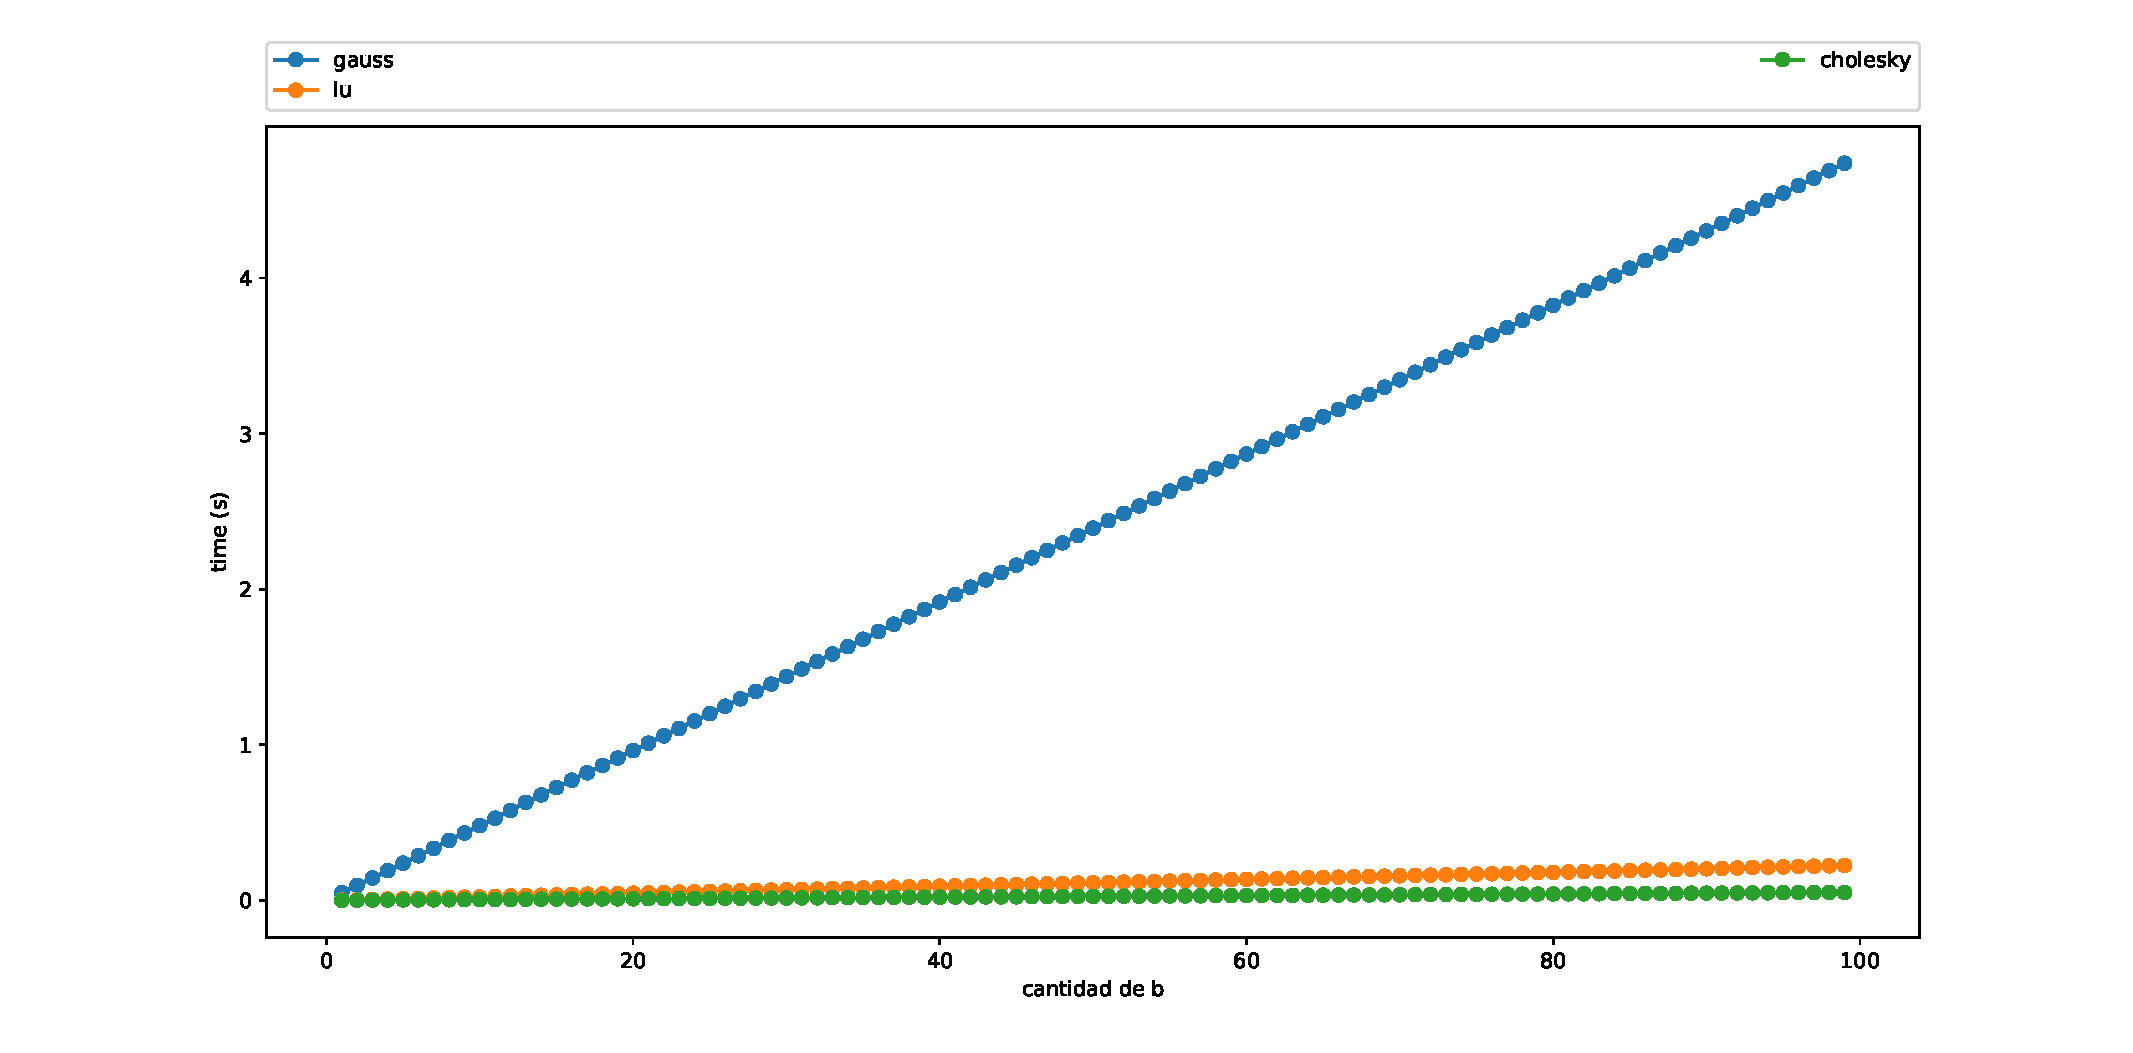
\includegraphics[scale=0.55]{informe/imagenes/tytalus/DistintosBSuma-Dim500.pdf}

Podemos observar en el gráfico que se cumple lo esperado. Algo quizá no contemplado es la pequeña diferencia de tiempos entre LU y Cholesky, que sospechamos fuertemente que está relacionada con la forma en que los implementamos.

% \hspace*{-2cm} \includegraphics[scale=0.5]{informe/imagenes/tytalus/DistintosBSuma-soloCholeskyLU-Dim500.pdf}



% {\centering
%     \includegraphics[scale=0.5]{informe/imagenes/tytalus/DistintosB-Dim500.pdf}
% }

% {\centering
%     \includegraphics[scale=0.5]{informe/imagenes/tytalus/DistintosB-soloCholeskyLU-Dim500.pdf}
% }


% -------------------------------------------------------
% Conclusiones
% -------------------------------------------------------
\newpage
\section{Conclusión}

En primer lugar vimos cómo calibrar el sistema para adaptarlo a cualquier ángulo de luz, obteniendo resultados similares a los provistos por la cátedra. \\

Resolvimos sistemas lineales para encontrar los vectores normales a la superfice. Lo hicimos utilizado el algoritmo de eliminación gaussiana. Luego nos aprovechamos de la estructura de nuestras ecuaciones para mostrar que existe la factorización LU y la utilizamos en nuestro problema. Comprobamos en la experimentación que LU es bastante más eficiente que Gauss, sin embargo, el tiempo que se tarda en el cálculo de normales se encuentra en el orden de los milisegundos para ambos métodos, mientras que el tiempo total se encuentra en el orden de los minutos, por lo que para nuestro problema es indistinto cuál usar. \\

Planteamos cómo sería un posible sistema matricial para el cálculo de profundidades a partir de las ecuaciones de los planos tangentes y vimos que cumplía ciertas propiedades. Para resolver el nuevo sistema, propusimos una nueva estructura de datos y resolvimos el sistema utilizando el algoritmo de Cholesky. \\

Finalmente, mostramos los resultados finales obtenidos y realizamos experimentaciones para entender mejor cómo se comporta nuestro sistema. Consideramos las diferencias que encontramos y concluimos que si bien no fue perfecto, aplicamos de manera satisfactoria la técnica de fotometría estéreo. \\

% -------------------------------------------------------
% Apéndice A
% -------------------------------------------------------
\newpage
\input{informe/Aappend.tex}

% -------------------------------------------------------
% Apéndice B
% -------------------------------------------------------
\newpage
\input{informe/Bappend.tex}

% -------------------------------------------------------
% Referencias
% -------------------------------------------------------
\newpage
\input{informe/ref.tex}


\newpage
\bibliographystyle{plain}
\bibliography{tp1}

\end{document}